% Vorlage für eine Bachelorarbeit
% Siehe auch LaTeX-Kurs von Mathematik-Online
% www.mathematik-online.org/kurse
% Anpassungen für die Fakultät für Mathematik
% am KIT durch Klaus Spitzmüller und Roland Schnaubelt Dezember 2011

\documentclass[12pt,a4paper]{scrartcl}
% scrartcl ist eine abgeleitete Artikel-Klasse im Koma-Skript
% zur Kontrolle des Umbruchs Klassenoption draft verwenden


% die folgenden Packete erlauben den Gebrauch von Umlauten und ß
% in der Latex Datei
\usepackage[utf8]{inputenc}

%\usepackage[latin1]{inputenc} %  Alternativ unter Windows
\usepackage[T1]{fontenc}
%\usepackage[ngerman]{babel}
%\usepackage{parskip}

%\usepackage{nicefrac}


\usepackage[pdftex]{graphicx}
\usepackage{latexsym}
\usepackage{amsmath,amssymb,amsthm}
\usepackage[disable]{todonotes}
\usepackage{float}



\usepackage{tikz}
\usetikzlibrary{automata,positioning}

% Abstand obere Blattkante zur Kopfzeile ist 2.54cm - 15mm
\setlength{\topmargin}{-15mm}

%\setlength{\parindent}{0pt}


% Umgebungen für Definitionen, Sätze, usw.
% Es werden Sätze, Definitionen etc innerhalb einer Section mit
% 1.1, 1.2 etc durchnummeriert, ebenso die Gleichungen mit (1.1), (1.2) ..
\theoremstyle{plain}
\newtheorem{Theorem}{Theorem}[section]
\newtheorem{Lemma}[Theorem]{Lemma}
\newtheorem{Remark}[Theorem]{Remark}

\theoremstyle{definition}
\newtheorem{Definition}[Theorem]{Definition}
\newtheorem{Notation}[Theorem]{Notation}
\newtheorem{Example}[Theorem]{Example}
	   
                  
\numberwithin{equation}{section} 

% einige Abkuerzungen
\newcommand{\C}{\mathbb{C}} % komplexe
\newcommand{\K}{\mathbb{K}} % komplexe
\newcommand{\R}{\mathbb{R}} % reelle
\newcommand{\Q}{\mathbb{Q}} % rationale
\newcommand{\Z}{\mathbb{Z}} % ganze
\newcommand{\N}{\mathbb{N}} % natuerliche
\newcommand{\2}{\mathbb{Z} / 2 \mathbb{Z}}
\newcommand{\G}{\mathcal{G}}
\newcommand{\1}{\bar{1}}
\newcommand{\0}{\bar{0}}
\newcommand{\widthrect}{160}
\newcommand{\widthrectb}{160}
\newcommand{\heightrect}{4}
\newcommand{\abstrect}{10}

\newcommand{\Aut}{\operatorname{Aut}}
\newcommand{\Bij}{\operatorname{Bij}}
\newcommand{\tr}{\operatorname{tr}}
\newcommand{\pr}{\operatorname{pr}}
\newcommand{\Homeo}{\operatorname{Homeo}}
\newcommand{\id}{\operatorname{id}}
\newcommand{\Ind}{\operatorname{Ind}}
\newcommand{\Mor}{\operatorname{Mor}}
\newcommand{\Ima}{\operatorname{Im}}
\newcommand{\Dom}{\operatorname{Dom}}

\renewcommand{\labelenumi}{\roman{enumi})}


\begin{document}
  % Keine Seitenzahlen im Vorspann
  \pagestyle{empty}

  % Titelblatt der Arbeit
  \begin{titlepage}

    
\includegraphics[scale=0.45]{kit-logo.jpg} 
    \vspace*{2cm} 

 \begin{center} \large 
    
    Masterarbeit
    \vspace*{2cm}

    {\huge Turing machines and irrational values of $\ell^2$-Betti numbers}
    \vspace*{2.5cm}

    Jan Kohlmüller
    \vspace*{1.5cm}

    20.08.2017
    \vspace*{4cm}


    Betreuung: Roman Sauer \\[1cm]
    Fakultät für Mathematik \\[1cm]
		Karlsruher Institut für Technologie
  \end{center}
\end{titlepage}



  % Inhaltsverzeichnis
  \tableofcontents

\newpage
 


  % Ab sofort Seitenzahlen in der Kopfzeile anzeigen
  \pagestyle{headings}

\section{Introduction}


\section{$\ell^2$-Betti numbers}
At first we will give a short introduction into the theory of $\ell^2$-Betti numbers. For a wider approach see \cite{LUECK}. We will assume some basic knowledge about cellular homology and the associated Betti numbers. For more information on this topic see e.g. \cite{HATCH}. As an alternative a reader not familiar with these topics may just accept the results of \ref{MCW} and study the definitions given in section \ref{fiss}.

In this whole chapter $G$ is always a discrete countable group with multiplication $\odot_G$.
\subsection{Von Neumann Dimension} \label{fiss}
At first let us begin with some basic definitions.
\begin{Definition} \label{GR}
	The \emph{group ring} $RG$ over a ring $R$ is the free module over $G$ with the additional multiplication
	\begin{align*}
		\sum_{h \in H} \alpha_h h \odot_{RG} \sum_{k \in K} \beta_k k = \sum_{h \in H} \sum_{k \in K} \alpha_h \beta_k h \odot_G k
	\end{align*}
	with $\alpha_h, \beta_k \in R$ and $H, K \in G$ finite subsets.
\end{Definition}
If $R$ is a field then $RG$ is an algebra and in particular a vector space with dimension $|G|$ if $G$ is finite. We will often see the group ring $\C G$. If $G$ is infinite then $\C G$ is an infinite dimensional vector space with scalar product. In this case $\C G$ is not a Hilbert space. Therefore we will introduce the space $\ell^2(G)$ which is in fact the Hilbert space completion of $\C G$.
\begin{Definition}
	$\ell^2(G)$ is the Hilbert space consisting of formal sums $\sum_{g \in G} \lambda_g g$ such that $\lambda_g \in \C$ and $\sum_{g \in G} |\lambda_g|^2 < \infty$. The multiplication is defined as in \ref{GR} and the scalar product is defined by
	\begin{align*}
		\langle \sum_{g \in G} \alpha_g g, \sum_{h \in G} \beta_h  h \rangle := \sum_{k \in G} \alpha_k \overline{\beta_k}.
	\end{align*}
\end{Definition}
\begin{Remark}
	If $G$ is a set instead of a group we can also define a Hilbert space $\ell^2(G)$. Of course we do not have a multiplication in this case.
\end{Remark}
We now want to define a dimension for spaces embedded in $\ell^2(G)$. In most cases the normal vector space dimension of these spaces will be infinite and therefore not useful. We will instead use the von Neumann dimension which requires some preliminary work.
\begin{Definition}
	The \emph{group von Neumann algebra} $\mathcal{N}(G)$ is defined as the algebra of (left-)$G$-equivariant bounded operators from $\ell^2(G)$ to $\ell^2(G)$ where $G$ acts on $\ell^2(G)$ by left multiplication.
\end{Definition}
We will denote the bounded operators of a Hilbert space $H_1$ by $\mathcal{B}(H_1)$. If $G$ acts on a Hilbert Space $H_2$ the subspace of $G$-equivariant elements of $H_2$ will be called $H_2^G$. Therefore we can also define the group von Neumann algebra by $\mathcal{N}(G) := \mathcal{B}(\ell^2(G))^G$.
\begin{Definition}
	Let $e_G \in G$ be the unit element of $G$. Then
	\begin{align*}
		\tr_{\mathcal{N}(G)}\colon \mathcal{N}(G) \to \C, A  \mapsto \langle A( e_G), e_G \rangle
	\end{align*}
	is called the \emph{von Neumann trace} on $\mathcal{N}(G)$.
\end{Definition}
\begin{Remark}
	Right multiplication with an element of the group ring $\C G$ is a $G$-equivariant operator on $\ell^2(G)$ and therefore has a well defined von Neumann trace. Note that left multiplication with an element of $\C G$ is not $G$-equivariant if $G$ is not abelian.
\end{Remark}
\begin{Definition}
	A \emph{Hilbert $\mathcal{N}(G)$-module} is a Hilbert space $H$ with a linear isometric $G$-action such that there exists an isometric linear $G$-embedding from $H$ to $\ell^2(G)^n$ for some $n \in \N$.
\end{Definition}
\begin{Definition}
	Let $H$ be a Hilbert $\mathcal{N}(G)$-module and let 
	\begin{itemize}
		\item $\iota\colon H \to \ell^2(G)^n$ be a corresponding embedding 
		\item $\pr_{\iota(H)}\colon \ell^2(G)^n \to H$ be a corresponding $G$-equivariant projection
		\item $\iota_i\colon \ell^2(G) \to \ell^2(G)^n, y \mapsto (0, \ldots, y \ldots 0)$ be the inclusion of the i-th $\ell^2(G)$
		\item $\pr_i\colon \ell^2(G)^n \to \ell^2(G), (x_1, \ldots, x_n) \mapsto x_i$  be the corresponding projection.
	\end{itemize}
	Then 
	\begin{align*}
		\tr_{\mathcal{N}(G)}\colon \mathcal{B}(H)^G \to \C, A \mapsto \sum_{i = 1}^{n} \tr_{\mathcal{N}(G)}(\pr_i \circ \iota \circ A \circ \pr_{\iota(H)} \circ \iota_i)
	\end{align*}
	is also called the \emph{von Neumann trace} on $H$.
\end{Definition}
One can show that the trace is independent of the chosen embedding and therefore well-defined.
\begin{Remark}
	A different way to understand the definition of the von Neumann trace on Hilbert $\mathcal{N}(G)$-modules is the following:
	A Hilbert $\mathcal{N}(G)$-module $H$ can always be seen as a $G$-equivariant subspace of some $\ell^2(G)^n$. A map $A \in \mathcal{B}(H)^G$ can then be expanded to a map on $\ell^2(G)^n$ by first projecting onto $H$ and then using $A$. In addition a map on $\ell^2(G)^n$ can be seen as a matrix of maps on $\ell^2(G)$.
	
	Taking the von Neumann trace of $A$ then simply means expanding $A$ to a map on $\ell^2(G)^n$ and then adding up the von Neumann trace of the diagonal entries of the matrix of this map.
\end{Remark}
\begin{Definition}\label{vNd}
	Let $H$ be a Hilbert $\mathcal{N}(G)$-module. We define the \emph{von Neumann dimension} of $H$ as
	\begin{align*}
		\dim_{\mathcal{N}(G)}(H) = \tr_{\mathcal{N}(G)}(\id_H).
	\end{align*}
\end{Definition}
\begin{Remark}\label{vNd_for_subsets}
	Let $H \subset \ell^2(G)$ be a subset which is closed under $G$ and $\pr_H\colon\ell^2(G) \to H$ a $G$-equivariant projection. Then\begin{align*}
	\dim_{\mathcal{N}(G)}(H) = \tr_{\mathcal{N}(G)}(\pr_H) = \langle \pr_H (e_G), e_G \rangle.
	\end{align*}
\end{Remark}

\subsection{$\ell^2$-Betti numbers of $G$-CW-complexes}
One can now define the $\ell^2$-Betti numbers of CW-complexes in a very similar way as for cellular homology. But first we have to define a group action on CW-complexes.
\begin{Definition}
	Let $X$ be a CW-complex and $\rho\colon G \to \Homeo(X)$ an action of $G$ on $X$ by homeomorphism such that for every open cell $E \subset X$ and every $g \in G$ it holds that $\rho(g)(E)$ is again an open cell and $\rho(g)|_{E} = \id_E$ if $\rho(g)(E) \cap E \neq \emptyset$. Then $\rho$ is called a \emph{cellular action}.
\end{Definition}

\begin{Definition}
	A \emph{$G$-CW-complex} is a CW-complex together with a cellular $G$-action.
\end{Definition}

\begin{Definition}
	The \emph{orbit} of an $n$-cell in a $G$-CW-complex is called a $G$-equivariant $n$-cell.
\end{Definition}

\begin{Definition}
	Let $X$ be a $G$-CW complex. $X$ is called
	\begin{itemize}
		\item \emph{proper} if all stabilizer groups are finite,
		\item \emph{free} if all stabilizer groups are trivial,
		\item \emph{finite type} if for every $n \in \N_0$ it has only finitely many $G$-equivariant $n$-cells.
	\end{itemize}
\end{Definition}

\begin{Remark}
	One can show that the chain complex of a $G$-CW complex $X$ is a chain complex $C_*(X)$ of left $\Z G$-modules, i.e. each $C_n(X)$ is a left $\Z G$-module and the differentials are $\Z G$- module-homomorphisms.
\end{Remark}
\begin{Definition}
	The \emph{$\ell^2$-chain complex} of a $G$-CW complex $X$ is
	\begin{align*}
		C_*^{(2)}(X) = \ell^2(G) \otimes_{\Z G} C_*(X).
	\end{align*}
\end{Definition}

\begin{Definition}
	Let $X$ be a proper, finite type $G$-CW complex and $C_*^{(2)}(X)$ the corresponding $\ell^2$-chain complex with its differential $d_*^{(2)}$. Then 
	\begin{align*}
		H_n^{(2)}(X) := \ker(d_n^{(2)}) / \overline{im(d_{n+1}^{(2)})}
	\end{align*}
	is called the \emph{$n$-th $\ell^2$-homology} and 
	\begin{align*}
		b_n^{(2)}(X)=\dim_{\mathcal{N}(G)}H_n^{(2)}(X)
	\end{align*}
	the \emph{$n$-th $\ell^2$-Betti number}.
\end{Definition}
\begin{Remark}
	One can show that for a proper, finite type $G$-CW complex $X$, the $n$-th $\ell^2$-homology $H_n^{(2)}(X)$ is a Hilbert $\mathcal{N}(G)$-module and therefore the $\ell^2$-Betti number is in fact well-defined.
\end{Remark}

\subsection{$\ell^2$-Betti numbers arising from a group}
We will now show that it is sufficient for our purpose to calculate the von Neumann trace of the kernel of elements of the group ring without mentioning CW-complexes.
\begin{Remark}\label{MAB}
	A matrix $A \in \C G^{n \times m}$ can be seen as an operator from $\ell^2(G)^n \to \ell^2(G)^m$ via $x \mapsto x^{\top} \cdot A$. We will refer to this map also by $A$. This operator is $G$-equivariant. Be aware that if $G$ is not abelian this is not the same operator as $A^\top x$, which in this case is not $G$-equivariant.
\end{Remark}
\begin{Lemma}
	For a matrix $A \in \C G^{n \times m}$ the kernel $\ker(A)$ is a Hilbert $\mathcal{N}(G)$-module and therefore has a well-defined von Neumann-dimension.
\end{Lemma}
\begin{proof}
	Of course $\ker(A)$ is a subspace of $\ell^2 (G)^n$. We can use $\id|_{\ker(A)}$ as embedding. It remains to show that $\ker(A)$ is closed under the natural $G$-action on $\ell^2 (G)^n$. So let $x \in \ker(A)$ be an element in the kernel and $g \in G$ be an element of the group. It now holds that
	\begin{align*}
		(g \cdot x)^\top \cdot A = g \cdot (x^\top A) = g \cdot 0 = 0
	\end{align*}
	because the action is linear.
\end{proof}
\begin{Theorem} \label{MCW}
	Let $x \in \R$ and $G$ be a discrete, countable, finitely generated group. The following are equivalent:
	\begin{enumerate}
		\item There exists a cocompact free finite type $G$-CW-complex $X$ and an integer $n \in \N$ such that $b_n^{(2)}(X)=x$.
		\item There exists a matrix $A \in \Q G^{n \times n}$ for an integer $n \in \N$ such that \newline $\dim_{\mathcal{N}(G)}(\ker (A))=x$.
	\end{enumerate}
\end{Theorem}
\begin{proof}
	$``i) \Rightarrow ii)''$ Let $X$ be a cocompact free finite type $G$-CW-complex and $l \in \N$ such that $b_l^{(2)}(X)=x$. We define 
	\begin{align*}
		\Delta_l^{(2)} = d_l^{(2)*} d_l^{(2)} + d_{l+1}^{(2)} d_{l+1}^{(2)*},
	\end{align*}
	which is a map from $C_l^{(2)}(X)$ to $C_l^{(2)}(X)$. The differential can be written as a matrix $A' \in \Z G^{n \times n}$ for some $n \in \N$ and therefore $\Delta_n^{(2)}$ also lies in $\Z G^{n \times n}$. In addition one can show that $\ker(\Delta_n^{(2)}) = H_n^{(2)}$ holds.
	
	$``ii) \Rightarrow i)''$ Let $n \in \N$ and $A\in \Q G^{n \times n}$. Because $k \cdot A$ has the same kernel as $A$ for every $k \in \Z$ we can assume that $A \in \Z G^{n \times n}$. The corresponding map will be also called $A$. We will construct a $G$-CW-complex $X$ with $d_3^{(2)} = A$ and $d_4^{(2)}$ trivial. Therefore $H_3^{(2)}(X) = \ker(A)$ and $i)$ follows.
	
	First we can see that a graph can always be seen as a CW-complex with the edges as 1-cells and the vertices as 0-cells. Let $g_1 \ldots g_m$ be generators of $G$ and let $Y$ be the corresponding Cayley graph of $G$ which has a natural cellular free $G$-action and is therefore a free, finite type $G$-CW-complex. In addition it has exactly one $G$-equivariant $0$-cell and $m$ $G$-equivariant $1$-cells and no other cells. We then glue $n$ many $2$-cells on each $0$-cell, i.e. we attach them via the attaching map which sends all of $S^1$ to a single point. For an example of this $G$-CW-complex with $G = \Z$ and $n = 2$ see Figure \ref{GCW_Grafik}.
	\begin{figure}[H]
		\centering
		\begin{tikzpicture}
		%	\shade[ball color = gray!40, opacity = 0.4] (0,0) circle (2cm);
		\draw (0,0) circle (1cm);
		\draw (-1,0) arc (180:360:1 and 0.3);
		\draw[dashed] (1,0) arc (0:180:1 and 0.3);
		\fill[fill=black] (0,-1) circle (2pt);
		
		\draw (0,-2) circle (1cm);
		\draw (-1,-2) arc (180:360:1 and 0.3);
		\draw[dashed] (1,-2) arc (0:180:1 and 0.3);
		
		\draw (3,0) circle (1cm);
		\draw (2,0) arc (180:360:1 and 0.3);
		\draw[dashed] (4,0) arc (0:180:1 and 0.3);
		\fill[fill=black] (3,-1) circle (2pt);
		
		\draw (3,-2) circle (1cm);
		\draw (2,-2) arc (180:360:1 and 0.3);
		\draw[dashed] (4,-2) arc (0:180:1 and 0.3);
		
		\draw (-3,0) circle (1cm);
		\draw (-4,0) arc (180:360:1 and 0.3);
		\draw[dashed] (-2,0) arc (0:180:1 and 0.3);
		\fill[fill=black] (-3,-1) circle (2pt);
		
		\draw (-3,-2) circle (1cm);
		\draw (-4,-2) arc (180:360:1 and 0.3);
		\draw[dashed] (-2,-2) arc (0:180:1 and 0.3);
		
		\draw[-] (0, -1) -- (-3, -1);
		\draw[-] (0, -1) -- (3, -1);
		
		\draw[dashed] (3, -1) -- (5, -1);
		\draw[dashed] (-3, -1) -- (-5, -1);
		
		\end{tikzpicture}
		\caption{An example of the $G$-CW-complex before gluing in the $3$-cells for $G = \Z$ and $n=2$.}
		\label{GCW_Grafik}
	\end{figure}
	
	We now glue in $n$ many $G$-equivariant $3$-cells in such a way that $A$ corresponds to $d_3^{(2)}$. We describe the procedure for the first row. The procedure for the other rows is done analogously.
	Let $A_{ij} = \sum_{g \in G} z_{(g, i, j)} g \in \Z G$ denote the entry in the i-th row and the j-th column of $A$. We fix one $0$-cell and call it $e$ and we call the corresponding $2$-cells $e_1 \ldots e_n$. We glue in $G \times D^3$ where each element $h \times D^3$ is glued $z_{(g, 1, j)}$ many times to $h g \cdot e_j$ for each $g \in G$ and $j \in \{1, \ldots, n\}$. We then see that $d_3^{(2)}$ maps the vector 
	\begin{align*}
		(\sum_{g \in G} \lambda_g g, 0 , \ldots , 0) \in (\ell^2 G)^n
	\end{align*}
	to
	\begin{align*}
		(\sum_{g \in G} \sum_{h \in H} \lambda_g z_{(h, 1, 1)} g h, \ldots , \sum_{g \in G} \sum_{h \in H} \lambda_g z_{(h, 1, n)}) \in (\ell^2 G)^.
	\end{align*}
	Figure \ref{GCW_Grafik2} shows how one $3$-cell $e \times D^3$ is glued on the above $G$-CW-complex for the first row of $A= \begin{pmatrix}
		1 \cdot 0 + 1 \cdot 2 & 1 \cdot 1 \\
		0 & 0
		\end{pmatrix}$. The $3$-cell is glued once into each of the gray $2$-cells.
		\begin{figure}[H]
			\centering
			\begin{tikzpicture}
			\shade[ball color = gray!40, opacity = 0.4] (-3,0) circle (1cm);
			\shade[ball color = gray!40, opacity = 0.4] (3,0) circle (1cm);
			\shade[ball color = gray!40, opacity = 0.4] (0,-2) circle (1cm);
			\draw (0,0) circle (1cm);
			\draw (-1,0) arc (180:360:1 and 0.3);
			\draw[dashed] (1,0) arc (0:180:1 and 0.3);
			\fill[fill=black] (0,-1) circle (2pt);
			
			\draw (0,-2) circle (1cm);
			\draw (-1,-2) arc (180:360:1 and 0.3);
			\draw[dashed] (1,-2) arc (0:180:1 and 0.3);
			
			\draw (3,0) circle (1cm);
			\draw (2,0) arc (180:360:1 and 0.3);
			\draw[dashed] (4,0) arc (0:180:1 and 0.3);
			\fill[fill=black] (3,-1) circle (2pt);
			
			\draw (3,-2) circle (1cm);
			\draw (2,-2) arc (180:360:1 and 0.3);
			\draw[dashed] (4,-2) arc (0:180:1 and 0.3);
			
			\draw (-3,0) circle (1cm);
			\draw (-4,0) arc (180:360:1 and 0.3);
			\draw[dashed] (-2,0) arc (0:180:1 and 0.3);
			\fill[fill=black] (-3,-1) circle (2pt);
			
			\draw (-3,-2) circle (1cm);
			\draw (-4,-2) arc (180:360:1 and 0.3);
			\draw[dashed] (-2,-2) arc (0:180:1 and 0.3);
			
			\draw[-] (0, -1) -- (-3, -1);
			\draw[-] (0, -1) -- (3, -1);
			
			\draw[dashed] (3, -1) -- (5, -1);
			\draw[dashed] (-3, -1) -- (-5, -1);
			
			\end{tikzpicture}
			\caption{The above example after gluing in one $3$-cell.}
			\label{GCW_Grafik2}
		\end{figure}
		
		
	We then repeat this for every row of $A$ and get that $d_3^{(2)} = A$. The resulting $G$-CW-complex $X$ is still free, finite type and because $X/G$ is finite $X$ is cocompact.
\end{proof}




\todo{ker(delta) = homology zeigen?}
\begin{Remark}
	One can show that \ref{MCW} also holds if $G$ is not finitely generated.
\end{Remark}
\begin{Definition}
	We say that a number $x \in \R$ \emph{arises} from a discrete countable group $G$ if it fulfills one (and therefore both) of the conditions of \ref{MCW}.
\end{Definition}
The statement of \ref{MCW} will be implicitly used in many points of this work. In fact we will never construct a $G$-Cw-complex and instead construct an element of a group ring $\Q (G)$ of $G$ which kernel has the desired von Neumann dimension.


\begin{Lemma}\label{add}
	If $x \in \R$ and $z \in \R$ both arise from a discrete, countable group $G$, then so does $x + z$.
\end{Lemma}
\begin{Lemma}\label{mult}
	Let $G$ is a discrete countable group and $H$ a discrete finite group. If $x \in \R$ arises from $G \times H$ then $x \cdot |H|$ arises from $G$.
\end{Lemma}
\todo{Vllt. noch beweisen oder Quelle}
\section{Turing dynamical systems}
To fix notation we will first give a definition of a Turing machine. For convenience we will only allow 1 and 0 as symbols on our tape.
\begin{Definition}
	A \emph{Turing machine} is a 5-tuple $T=(S,\delta, A, R, I)$ where S is a finite set of states and 
	\begin{align*}
		\delta\colon\2 \times S \setminus(A \cup R) \to \2 \times \{-1, 0, 1\} \times S
	\end{align*}
	is called the transition function. $A \subset S$ is called the set of accepting states, $R \subset S$ is called the set of rejecting states and $I \in S$ is called the initial state.
	A Turing machine is \emph{read-only} if $\delta$ fixes the $\2$-coordinate, i.e.
	\begin{align*}
		\delta (x, \sigma) = (x, \beta, \tilde{\sigma})
	\end{align*}
	for each $x \in \2$ and $\sigma \in S \setminus(A \cup R)$.
\end{Definition}
In addition each Turing machine uses a ``tape'', i.e. a set $\Z / 2\Z ^{\Z}$ with a ``head'' on the element corresponding to the index 0. A Turing machine can operate on an element of $Y \in \Z / 2\Z ^{\Z}$ which is called an input. We start with the initial state and use the transition function $\delta$ to get $\delta(Y_0, I)$. The first coordinate corresponds to the new element $Y_0$, the third to the new state and the second corresponds to shifting the tape to the left or the right and therefore getting a new $Y_0$, e.g. if $\delta(I, Y_0)_3 = 1$ we shift the whole tape one to the left, therefore our new $Y_0$ is our old $Y_1$. We repeat this step until we get a state in $A \cup R$. We say that the Turing machine accepts $Y$ if we get a state in $A$ after finitely many steps and it rejects $Y$ if we get a state in $R$ after finitely many steps. We say that the Turing machine holds for $Y$ if it accepts or rejects it.

For the purpose of calculating $\ell^2$-Betti numbers of groups we need to extend this definition. 
Let
\begin{itemize}
	\item $(X, \mu)$ be a probability measure space,
	\item $\bigcup_{i} X_i$ be a division of $X$ into finitely many disjoint measurable subsets,
	\item $\Gamma$ be a countable discrete group,
	\item $\rho$ be a right measure preserving action of $\Gamma$ on X,
	\item $A$, $R$ and $I$ be three disjoint subsets where each of them is a union of certain $X_i$. They will be called the accepting set, the rejecting set and the initial set.
	\item $\gamma_i \in \Gamma$ for each $X_i \subset X$ such that for each $i$ with $X_i \subset A$ or $X_i \subset R$ it holds that $\gamma_i = e$ where $e$ is the neutral element in $\Gamma$.
\end{itemize}
Let $\Ind\colon X \to \N$ be the index map, i.e the map for which
\begin{align*}
	\Ind(x) = i ~\Leftrightarrow~ x \in X_i
\end{align*}
holds.
\begin{Definition}
	 The map 
	 \begin{align*}
	 T_X\colon X \to X, x \mapsto \rho(\gamma_{\Ind(x)})(x)
	 \end{align*}
	 is called the \emph{Turing map}.
	 The group $\Gamma$ and the space $X$ (with all the choices of subsets and corresponding $\gamma_i$ made in the last paragraph) together with the Turing map will be called a \emph{Turing dynamical system} and will be denoted by $(T_X)$
\end{Definition}
Let $x \in X$. If there is a $k \in \N$ such that $T_X^k(x) = T_X^{k + 1}(x)$, then it also holds that $T_X^h(x) = T_X^{h + 1}(x)$ for all $h \in \N$ with $h \geq k$. We then define $T_X^\infty (x) := T_X^k(x)$. Mostly we don't look at the map $T_X$ but the map $T_X^\infty$. We say that the Turing dynamical system $(T_X)$ accepts an input $y \in I$ if $T_X^\infty(y) \in A$ and it rejects it if $T_X^\infty(y) \in R$. In addition we say that $(T_X)$ holds for $y$ if it accepts or rejects it.

For every Turing machine there is a Turing dynamical system which does the same as the Turing machine. More precisely for every Turing machine $T$ we can construct a Turing dynamical system $(T_X)$ and a bijection $\Psi\colon\2^\Z \to I$ such that $T$ accepts (rejects) an input $Y \in \2^\Z$ if and only if $(T_X)$ accepts (rejects) $\Psi(Y)$. We will use this fact may times in chapter \ref{chlamplighter}. The following example shows how the corresponding Turing dynamical system is constructed. But first let us fix notation.
\begin{Notation} \label{notation_TM}
	For a set $N$, let $k,l \in \N$ and $ (m_{-k}, \cdots,  m_l) \in N^{k+l+1}$. 
	
	Then let $M \subset N^\Z$  be defined by 
	\begin{align*}
		M := \{(n_i)_{i \in \Z} \in N^\Z | n_{-k} = m_{-k}, \cdots, n_l = m_l \},
	\end{align*}
	i.e. a set where $k+l +1$ coordinates including the $0$-coordinate are fixed. We then simply write $[m_{-k} \cdots \underline{m_0} \cdots m_l]$ for $M$ and $[m_{-k} \cdots \underline{m_0} \cdots m_l][\sigma]$ for $M \times \{\sigma\}$.
\end{Notation}
\begin{Example}\label{TMtoTDS}
	Let  $T=(S,\delta, \tilde{A}, \tilde{R}, \tilde{I})$ be a Turing machine. We define $X := \2^\Z \times S$ and $\Gamma := \2 \times \Z \times \Bij(S)$.
	The action of $\Gamma$ on $X$ is defined by the following rules:
	\begin{itemize}
		\item The generator $\1$ of the group $\Z / 2\Z$ acts on the $\Z / 2\Z^\Z$ part of $X$ by adding $\1$ to the element with index $0$.
		\item The generator $1$ of the group $\Z$ acts also on the $\Z / 2\Z^\Z$ part by shifting every element 1 to the left, i.e. decreasing the index of every element by 1.
		\item $\Bij(S)$ acts on $S$ in the natural way.
	\end{itemize}
	We will now use the transition function to construct the Turing map. We choose the following division of $X$:
	\begin{align*}
	X = \bigcup_{x \in \2, \sigma \in S} [\underline{x}][\sigma].
	\end{align*}
	For an arbitrary $X_i = [\underline{x}][\sigma]$ we can use the transition function of the Turing machine. Let
	\begin{align*}
		(\alpha, \beta,\hat{\sigma}) := \delta(x, \sigma) \in \2 \times \{-1, 0, 1\} \times S
	\end{align*} 
	denote  the image of $(x, \sigma)$. \\
	Now let $\tau \in \Bij(S)$ be some map which sends $\sigma$ to $\hat{\sigma}$. We can see $x-\alpha \in \2$ as a map on $\2$ which sends $x$ to $\alpha$. Our element $\gamma_i$ corresponding to $X_i$ is then given by 
	\begin{align*}
		\gamma_i := \begin{cases}
			(\0, 0, \id) & ~\text{if}~ X_i \subset A \cup R \\
			(x-\alpha, \beta, \tau) & ~\text{otherwise}
		\end{cases}.
	\end{align*} 
	Now we only need to define $A$, $R$ and $I$. $A$ is given by
	\begin{align*}
	A := \bigcup_{x \in \2, \sigma \in \tilde{A}}[\underline{x}][\sigma]
	\end{align*}
	which is of course a union of some $X_i$. $R$ and $I$ can be defined analogously. 
	
	The resulting Turing dynamical system $(T_X)$ accepts (rejects) an element in the initial set $Y \times \{\tilde{I}\} \subset I$ if and only if the Turing machine $T$ accepts (rejects) the input $Y \in \2^\Z$.
\end{Example} \todo{A und R nur ein Zustand}
Our ultimate goal is to use Turing dynamical systems to get $\ell^2$-Betti numbers arising from a group. For this purpose some additional definitions and restrictions are needed. \todo{praeziser}
\begin{Definition}
	The \emph{first fundamental set} $\mathcal{F}_1(T_X)$ is the subset of $I$ consisting of those points $x$ with $T_X^\infty(x) \in A$ such that there is no point $y$ with $T_X(y)=x$. The \emph{second fundamental set} is the subset of $A$ defined as $\mathcal{F}_2(T_X)=T_X^\infty(\mathcal{F}_1(T_X))$. The \emph{first (second) fundamental value} $\Omega_1(T_X) \ ( \Omega_2(T_X))$ is the measure of the corresponding fundamental set.
\end{Definition}

\begin{Definition}
	We say that a Turing dynamical system $(T_X)$
	\begin{itemize}
		\item \emph{stops on any configuration} if $T_X^\infty (x) \in A \cup R$ for almost all $x \in X$,
		\item \emph{has disjoint accepting chains} if $T_X^\infty (x) \neq T_X^\infty (y)$ for almost all $x, y \in \mathcal{F}_1(T_X)$ with $x \neq y$,
		\item \emph{does not restart} if the set $T_X(X) \cap I$ has measure $0$.
	\end{itemize}
\end{Definition}
 

\begin{Definition}
	Let $(T_X)$ be a Turing dynamical system such that $X$ is an infinite product of $\2$, i.e. $X$ is of the form $ \Pi_{j \in J} \2$. In addition, $X$ is equipped with the normalized (left) Haar measure and each $X_i$ is of the form 
	\begin{align*}
		X_i = \{(x_j)_{j \in J} \in X \ | \ x_k = \0 \ \forall k \in I_0, x_h = \1 \ \forall h \in I_1\}.
	\end{align*}
	where $I_0, I_1 \subset J$ are finite subsets.
	If in addition
	\begin{itemize}
		\item the action of $\Gamma$ is by continuous group automorphisms
		\item $(T_X)$ stops on any configuration
		\item $(T_X)$ has disjoint accepting chains
		\item $(T_X)$ does not restart
	\end{itemize}
	$(T_X)$ is called a \emph{computing} Turing dynamical system.
\end{Definition}
\begin{Remark}
	For more information on Haar measure see e.g. \todo{Quelle fuer Haar measure}. For us it is only relevant that there always exists a unique normalized (left) Haar measure on $G$ if $G$ is a locally compact Hausdorff topological group.
	
	Nate that the (left) Haar measure is left translation invariant.
\end{Remark}
\begin{Lemma}
	Let $(T_X)$ be a computing Turing dynamical system with $X = \Pi_{j \in J} \2$ and equipped with the normalized Haar measure $\mu$. For a set 
	\begin{align*}
		M = \{(x_j)_{j \in J} \in X \ | \ x_k = \0 \ \forall k \in I_0, x_h = \1 \ \forall h \in I_1 \}
	\end{align*}
	with $I_1, I_2 \subset J$ it holds that
	\begin{align*}
	\mu (M) = \begin{cases}
	\frac{1}{2^{|I_0| \cdot |I_1|}} & ~\text{if $I_0$ and $I_1$ are finite} \\
	0 & ~ \text{if $I_0$ or $I_1$ is infinite}
	\end{cases}.
	\end{align*}
\end{Lemma}
\begin{proof}
	Let $x \in X$ be an element with $\0$ on every coordinate $i \notin I_0 \cup I_1$ and $\1$ on at least one coordinate $i \in I_0 \cup I_1$. Then $xM$ and $M$ are disjoint and because of the left translation invariance of the measure it holds that $\mu (M) = \mu (xM)$. Because for every $i \in I_0 \cup I_1$ we can set the corresponding coordinate either to $\1$ or to $\0$ we get $2^{|I_0| \cdot |I_1|}$ of these sets if $I_0$ and $I_1$ are finite and an infinite amount of sets if one of them is infinite. The disjoint union of all of these sets is the whole set $X$ so the sum of these measures equals 1 and the claim follows.
\end{proof}
 
Before we give an example of a computing Turing dynamical system we fix the notation of the shifting operation, because we will need it later on.
\begin{Definition} \label{shift}
	An element $z \in \Z$ acts on $\2^{\Z} = \prod_{i \in \Z} \2$ by decreasing every index by $z$. We call this action the \emph{shift action} and denote it by $\zeta$. $\Z$ acts on $\bigoplus_{i \in \Z} \2$ in the same way and this operation will also be called $\zeta$.
\end{Definition}
Of course the Turing dynamical system constructed in \ref{TMtoTDS} is not computing in most cases. But for many read-only Turing machines a computing Turing dynamical system can be constructed in a similar way.\footnote{A computable Turing dynamical system can also be constructed for non read-only Turing machines in a different way as in \ref{TMtoTDS}. The main problem here is that adding $\1$ to the element of $\2^\Z$ with index $0$ is not a group-homomorphism.} In fact we will only use read-only Turing machines.
\begin{Example} \label{roTMtoTDS}
	Let $T$ be a read-only Turing machine, such that the corresponding Turing dynamical system $(T_X)$ as constructed in \ref{TMtoTDS} has disjoint accepting chains and stops on any configuration.\footnote{This is not the case for all read-only Turing machines.}
	
	We will construct a computable Turing dynamical system from $T$.  We can easily assure that $(T_X)$ does not restart by adding a new state $I'$ to $T$ with $\delta(x, I') = \delta(x, I)$ for all $x \in \{ \0, \1 \}$ and setting $I'$ as the initial state of $T$.
	
	Because we do not change the symbols of the tape it suffices to use $\Gamma = \Z \times \Bij(S)$ where $\Z$ operates on the $\2^\Z$ part via shifting and $\Bij(S)$ acts on $S$ in the natural way. Because a Turing machine has only finitely many states there exists an integer $n \in \N$ such that $|S| < 2^n$. We identify every state with a different element $z \in \2^n$ with $z \neq 0$.
	
	We can then assume that $X = \2^\Z \times \2^n$. We regard every element of $\2^n$, which does not correspond to an actual state, as a ``dummy state'' which will never be used. Because $\Aut(\2^n)$ acts transitively on all of $\2^n \setminus \{0\}$ we can choose our bijections on $S$ to be group automorphisms. Then $\gamma_i \in \Z \times \Aut(S)$ and therefore we may set $\Gamma := \Z \times \Aut(S)$. It acts on $X$ by continuous group automorphisms.
	
	In this case the sets $X_i = [\underline{x}][\sigma]$ as constructed in \ref{TMtoTDS} have only $n+1$ fixed components, one component to fix $x$ and $n$ components to fix $\sigma$. Therefore these sets are of the desired form.
	 
	It follows that the resulting Turing dynamical system is computing.
\end{Example}

\section{Computing $\ell^2$-Betti numbers}
In this chapter we want to prove the following central theorem which connects $\ell^2$-Betti numbers to the concept of Turing dynamical systems.
\begin{Theorem} \label{HS}
	Let $(T_X)$ be a computing Turing dynamical system. Then $\mu (I) - \Omega_1(T_X)$ is an $\ell^2$-Betti number arising from the group $\hat{X} \rtimes_{\hat{\rho}} \Gamma$ where $\hat{X}$ and $\hat{\rho}$ are the Pontryagin duals of the corresponding group or map.
\end{Theorem}
We will give the definition of Pontryagin duals and the semidirect product later in this chapter. The rest of this chapter is used to prove this theorem and give the needed definitions.

Figure \ref{Masterplan} shows our procedure to prove this Theorem. The main effort will be the proof of Theorem \ref{groserSatz}.

\begin{figure}[H]
	\centering
	\begin{tikzpicture}[shorten >=1pt,on grid,auto]
		\node[draw, rectangle, minimum width = \widthrect] (0) {Turing machine ($T$)};
		\node[draw, rectangle, minimum width = \widthrect] (1) [below = \heightrect of 0] {Turing dynamical system ($(T_X)$)};
		\node[draw, rectangle, minimum width = \widthrect] (2) [below = \heightrect of 1] {Groupoid ($\G(\rho)$)};
		\node[draw, rectangle, minimum width = \widthrect] (3) [below = \heightrect of 2] {Group ring ($\hat{X} \rtimes_{\hat{\rho}} \Gamma$)};
		\node[draw, rectangle, minimum width = \widthrect] (4) [below = \heightrect of 3] {$(\hat{X} \rtimes_{\hat{\rho}} \Gamma)$-CW-complex};
		\node[draw, rectangle, minimum width = \widthrectb, text width = \widthrectb, align = center] (5) [right =\abstrect of 1] {$x :=\mu(I) - \Omega_1(T)$ can be computed};
		\node[draw, rectangle, minimum width = \widthrectb, text width = \widthrectb, align = center] (6) [right =\abstrect of 2] {there exists an element $S$ in the groupoid ring with $\dim_{\mathcal{N}(G)}(\ker S) = x$};
		\node[draw, rectangle, minimum width = \widthrectb, text width = \widthrectb, align = center] (7) [right =\abstrect of 3] {there exists an element $S'$ in the group ring with $\dim_{\mathcal{N}(G)}(\ker S') = x$};
		\node[draw, rectangle, minimum width = \widthrectb, text width = \widthrectb, align = center] (8) [right =\abstrect of 4] {$x$ arises from a group (namely from $\hat{X} \rtimes_{\hat{\rho}} \Gamma$)};
		\path[dashed, ->]
			(1) edge [text width = 5 cm]
				node {taking the action groupoid as defined in \ref{action_groupoid}} 
				(2)
			(2) edge [text width = 5 cm]
				node {using the map $P \otimes 1$ as defined in \ref{map_pantryagin}}
				(3)
			(3) edge [text width = 5 cm]
				node{constructing a $G$-CW-complex as done in the proof of \ref{MCW}}
				(4)
		;
		\path[->]
			(0) edge [text width = 5 cm]
				node {Constructing the corresponding Turing dynamical system as done in \ref{roTMtoTDS}}
				(1)
			(1) edge [text width = 5 cm]
				node {}
				(5)
			(5) edge [text width = 5 cm]
				node {using the fact proven in \ref{groserSatz}}
				(6)
			(6) edge [text width = 5 cm]
				node {using that $S$ lies in the image of $P \otimes 1$ as proven in \ref{image_of_P}}
				(7)
			(7) edge [text width = 5 cm]
				node {using the fact proven in \ref{MCW}}
				(8)
		;
	\end{tikzpicture}
	\caption{Procedure to get an $\ell^2$-Betti number out of a Turing machine.}
	\label{Masterplan}
\end{figure}

\subsection{Groupoids}
We begin by giving some algebraic definitions, namely the construct of groupoids which extends the definition of groups. Therefore we require some basic knowledge about categories. \todo{Quelle zu Kategorientheorie}
\begin{Definition}
	A \emph{groupoid} is a small category whose morphisms are all invertible.
\end{Definition}
\begin{Example} \label{group}
	Let $G$ be a group. We want to see how we can express $G$ as a groupoid. Let $\mathcal{G}_0 = \{\bullet\}$ be the set with only one element  and $\mathcal{G}$ be the category with objects $\G_0$ and morphisms $\Mor(\bullet, \bullet) = G$. The composition of morphisms in $\mathcal{G}$ is the same as the multiplication in $G$. Then $\mathcal{G}$ is a small category and every morphism is invertible because every group element has an inverse. Therefore $\mathcal{G}$ is a groupoid.
\end{Example}
We will always denote the set of objects of a groupoid $\mathcal{G}$ by $\mathcal{G}_0$ and we can identify it with a subset of the set of morphisms of $\mathcal{G}$ by the embedding 
\begin{align*}
	\mathcal{G}_0 \to \Mor(\mathcal{G}), X \mapsto [\id\colon X \to X]
\end{align*}
which sends every object to the corresponding identity morphism. Therefore we will only only look at $\Mor(\mathcal{G})$ and also call it $\mathcal{G}$. 

We will now give some definitions of basic properties of groupoids which we will use later in this chapter.

\begin{Definition}
	For every groupoid $\mathcal{G}$ we define the maps
	\begin{align*}
		s\colon \mathcal{G} \to \mathcal{G}_0, [f\colon X \to Y] \mapsto X
	\end{align*}
	and
	\begin{align*}
		r\colon\mathcal{G} \to \mathcal{G}_0, [f\colon X \to Y] \mapsto Y
	\end{align*}
	which will be called \emph{source} and \emph{range} map.
\end{Definition}
\begin{Definition}
	A \emph{relation groupoid} is a groupoid with 
	\begin{align*}
		|\Mor(X, Y)| \leq 1 \ \forall X,Y \in \G_0.
	\end{align*}
\end{Definition}
\begin{Remark}
	There is a one-to-one correspondence between relation groupoids and equivalence relations.
\end{Remark}

\begin{Definition}
	If $X \in \G_0$ we denote by $\G X \subset \G_0$ the set of all those objects $Y \in \G_0$ with $\Mor(X, Y) \neq \emptyset$ and call it the \emph{orbit} of $X$.
\end{Definition}

Our main use of groupoids will be to construct a groupoid out of a Turing dynamical system (see Figure \ref{Masterplan}). Therefore we consider groupoids which are also measurable spaces: 
\begin{Definition}\label{discr_meas}
	A \emph{discrete measurable groupoid} is a groupoid where $\mathcal{G}$ is also a measurable space, $s, r$ and the maps gained by inverting or composition are all measurable and the fibers of $s$ and $r$ are countable.
	
	If in addition we have a measure $\mu$ such that for every $U \subset \mathcal{G}$
	\begin{align*}
		\int_{\mathcal{G}_0} |r^{-1}(x) \cap U| ~d\mu(x) = \int_{\mathcal{G}_0} |s^{-1}(x) \cap U| ~d\mu(x) 
	\end{align*}
	holds, we call $\mathcal{G}$ \emph{discrete measured}.
\end{Definition}
\todo{Warum braucht man das eigentlich nochmal, was bedeutet das genau und stimmt das eigentlich? inverting map, mu auf G}
From now on every groupoid will be discrete measured.
\begin{Definition}
	We say that a groupoid $\G$ has \emph{finite orbits} if $\G X$ is finite for almost all $X \in \G_0$.
\end{Definition}
\begin{Definition}
	Let $\G$ be a relation groupoid with finite orbits. A measurable subset $D \subset \G_0$ such that $|D \cap \G X| = 1$ for every $X \in \G$ with $\G X$ finite is called a \emph{fundamental domain}.
\end{Definition}
\begin{Remark}
	Up to null-sets a fundamental domain $D$ is an inclusion-minimal subset of $\G_0$ such that $\G D = \G_0$.
\end{Remark}
\begin{Remark}
	One can show that every relation groupoid with finite orbits has a fundamental domain.
\end{Remark}


\subsection{Groupoid ring}
A fundamental concept used for the calculation of $\ell^2$-Betti numbers of groups was the group ring. We will transfer this to the notion of groupoids.

\begin{Definition}
	Let $U$ be a subset of $\G_0$. A \emph{measurable edge} is a map $\Phi\colon U \to \G$ such that $s \circ \Phi = \id$ and $r \circ \Phi$ is injective.
\end{Definition}
\todo{Warum heißt das eigentlich messbar?}
From the definition we see, that defining a measurable edge means taking a subset of $\G_0$ and associating a morphism to every object such that the morphism starts in this object and no two such morphisms end in the same object. We want to define the inverse of a measurable edge in such a way, that it is also a measurable edge. Therefore it does not suffice to take the inverse of the map $\Phi$. Instead we invert each morphism in the image of $\Phi$.
\begin{Definition}
	Let $\Phi\colon U \to \G$ be a measurable edge. The \emph{inverse} of $\Phi$ will be called $\Phi^{-1}$ and is defined as \begin{align*}
		\Phi^{-1}\colon r(\Ima(\Phi)) \to \G, x \mapsto \Phi (y)^{-1}
	\end{align*}
	where $y$ is the unique element in the preimage $(r \circ \Phi)^{-1} (x)$ and $\Phi (y)^{-1}$ is the inverse of the morphism $\Phi (y)$.
\end{Definition}\todo{Anschauung}

We now come to the definition of the groupoid ring. We want it to be a ring of operators on	$L^2(\G)$, \todo{Quelle fuer l2} such that it is in a way generated by measurable edges.
\begin{Definition}\label{groupoid_ring}
	For a measurable edge $\Phi$ we define an operator $\tilde \Phi$ by
	\begin{align*}
	\tilde \Phi\colon L^2(\G) \to L^2(\G), F \mapsto \left[\gamma \mapsto \begin{cases}
	F(\gamma \odot_{\G} \Phi^{-1}(r(\gamma)) & \text{if } r(\gamma) \in \Dom(\Phi^{-1}) \\
	0 & \text{otherwise}
	\end{cases} \right] .
	\end{align*}
	\todo{da sollte man ein Bild zu malen}
	In addition for a map $f \in L^\infty (\G_0)$ we also define an operator $\tilde f$ on $L^2(\G)$ by
	\begin{align*}
	\tilde f\colon L^2(\G) \to L^2(\G), F \mapsto [\gamma \mapsto F(\gamma) \cdot f(r(\gamma))].
	\end{align*}
	For a groupoid $\G$ the \emph{groupoid ring} $\C\G$ is the ring of bounded operators on $L^2(\G)$ generated by all $\tilde{\Phi}$ with $\Phi$ measurable edge and all $\tilde{f}$ with $f \in L^\infty(\G_0)$.
\end{Definition}
We always denote the elements of $\C\G$ by a linear combination $\sum_{i \in I} \tilde \Phi_i \odot_{\C \G} \tilde f_i$ where $I$ is a finite set, $\Phi_i$ is a measurable edge and $f_i \in L^\infty(\G_0)$. One can show that each element of $\C \G$ can be represented in such a way. Be aware that this representation is non-unique because there might be several pairs of operators such that their respective compositions are equal. In addition for $f \in L^\infty(\G)$ it holds that $\widetilde{\frac{1}{2}f} + \widetilde{\frac{1}{2}f} = \tilde{f}$. \todo{Evtl. könnte ich dazu noch ein bisschen was schreiben}
\begin{Example} \label{groupoid_ring_of_groups}
	Let $G$ be a group and $\G$ the corresponding groupoid as in Example \ref{group}. We want to show that the groupoid ring $\C \G$ as a ring is isomorphic to the group ring $\C G$. Because there is only one element in $\G_0$ the only measurable edges are the maps from $\{\bullet\}$ to $G$ (as a set). The elements of $L^\infty(\G_0)$ are just maps from $\{\bullet \}$ to $\C$. Therefore  $L^\infty(\G_0)$ is isomorphic to $\C$. 
	
	We now need to show that the composition on $\{\tilde{\Phi}~|~ \Phi~\text{measurable edge}\}$ agrees with the composition on $G$.
	On our measurable edges we define the isomorphism: For a measurable edge $\Phi\colon\bullet \mapsto g$ we map $\tilde{\Phi}$ to $g$. This map is of course bijective. To see that it is a homomorphism let $\Phi_1\colon\bullet \mapsto g_1$ and $\Phi_2\colon\bullet \mapsto g_2$ be measurable edges. It follows that
	\begin{align*}
		  &~ (\tilde{\Phi}_1 \odot_{\C \G} \tilde{\Phi}_2)(F)(\gamma) \\
		= &~ (\tilde{\Phi}_2 \circ \tilde{\Phi}_1)(F)(\gamma) \\
		= &~ \tilde \Phi_2 (\alpha \mapsto F(\alpha \odot_{\G}\Phi_1^{-1}(\bullet)))(\gamma) \\
		= &~ F((\gamma \odot_{\G} \Phi_2^{-1}(\bullet)) \odot_{\G} \Phi_1^{-1}(\bullet)) \\
		= &~ F(\gamma \odot_G g_2^{-1} \odot_G g_1^{-1}) \\
		= &~ F(\gamma \odot_G (g_1 \odot_G g_2)^{-1}) \\
		= &~ \tilde{\Psi} (F)(\gamma)
	\end{align*}
	where $\Psi$ is the measurable edge $\bullet \mapsto g_1 \odot_G g_2$.
\end{Example}


\subsection{Groupoids of Turing dynamical systems}
We can now define the action groupoid which will allow us to create a groupoid from a Turing dynamical system.
\begin{Definition} \label{action_groupoid}
	Let $\Gamma$ be a discrete, countable group, $X$ a probability measure space and $\rho\colon\Gamma \to \Bij(X)$ a right measure preserving action.
	
	The \emph{action groupoid} $\G(\rho)$ is the groupoid with objects $X$ and morphisms $X \times \Gamma$ such that $(x,\gamma)$ is a morphism $x \to \rho(\gamma)(x)$. The composition of morphisms is defined by
	\begin{align*}
		(x, \gamma_1) \odot_{\G(\rho)} (\rho(\gamma_1) (x), \gamma_2) = (x, \gamma_1 \odot_\Gamma \gamma_2).
	\end{align*}
\end{Definition}

\begin{Remark} \label{mE_action_groupoid}
	Let $\G(\rho)$ be an action groupoid of the action $\rho \colon \Gamma \to \Bij(X)$. For each element $\gamma \in \Gamma$ we get a measurable edge $\bar{\gamma}\colon X \to X \times \Gamma$ which maps $x \in X$ to $(x, \gamma)$.
\end{Remark}



\begin{Remark}
	If $(T_X)$ is a Turing dynamical system with group action $\rho$, then the action groupoid $\G(\rho)$ is a discrete measured groupoid (as defined in Definition \ref{discr_meas}).
\end{Remark}
\todo{warum discrete measured?}
\begin{Definition}
	Let $(T_X)$ be a Turing dynamical system with group action $\rho$. Then $\G (T_X) \subset \G(\rho)$ is the smallest groupoid with $\G (T_X)_0 = \G(\rho)_0$, which contains all morphisms of the form $(x, \gamma_i)$ where $i = \Ind(x)$ is the index of the $X_i$ that $x$ is contained in.
\end{Definition}
\begin{Lemma} \label{TX_rel_groupoid}
	$\G (T_X)$ is a relation groupoid with finite orbits for every computing Turing dynamical system $(T_X)$. In addition $A \cup R$ is a fundamental domain of $\G (T_X)$.
\end{Lemma}
\begin{proof}
	First let us have a look at $\G (T_X)$. Its objects are $\G_0 = X$. We then add all morphisms of the form $(x, \gamma_{\Ind(x)})$. We call the subset we have created so far $\G'$. Of course $\G'$ will usually not be a category. Now we take the smallest groupoid which contains $\G'$: We add a morphism from $x$ to $y$ for all $x, y \in \G_0$ where there already exist a path of morphisms from $x$ to $y$ in $\G'$. In addition we add an identity morphism to every $ x\in \G_0$ which does not already have one and an inverse morphism to every morphism which does not already have one. 
	
	We can then see that we get one morphism from $x$ to $y$ in $\G (T_X)$ for every path of morphisms from $x$ to $y$ in $\G'$. But $x$ has exactly one outgoing morphism in $\G'$, therefore $\G (T_X)$ is a relation groupoid.

	Because $(T_X)$ stops on any configuration there has to be a path of morphisms in $\G'$ from $x$ to a unique point in $A \cup R$ for almost any $x \in \G (T_X)_0$. Therefore the orbit $\G (T_X)x$ of almost any point $x \in \G (T_X)$ contains exactly one point in $A \cup R$ and $A \cup R$ is a fundamental domain.
	
	To prove that $\G (T_X)$ has finite orbits we restrict the groupoid $\G (T_X)$ to a groupoid $\G (T_X)^\#$ by restricting the objects to those objects $x$ with $\G (T_X)x \cap (A \cup R) \neq \emptyset$. Because $(T_X)$ stops on any configuration, $\G (T_X)^\#$ still has measure $1$.
	
	For $i \in \N_0$, we define the set $Y_i \subset \G (T_X)_0^\#$ to be the set of points, such that for every point $y \in Y_i$ there is an acyclic path of length $i$ in $\G'$ from $y$ to a point in $A \cup R$, i.e. $T_X^i(y) \in A \cup R$ and $T_X^{i-1} \notin A \cup R$. These sets are disjoint and measurable because $T_X$ is measurable and therefore $\sum_{i \in \N_0} \mu(Y_i) = 1$. Therefore $\mu(Y_i)$ has to be a zero sequence.
	
	Now consider the set 
	\begin{align*}
		Y := \{y \in A \cup R ~|~ \G y ~ \text{is infinite}\}. 
	\end{align*}
	A Turing dynamical system has only finitely many sets $X_i$ and therefore each point has only finitely many pre-images. Because $T_X^i(Y_i) \subset T_X^{i-1}(Y_{i-1})$ it holds that $Y$ equals $\bigcap_{i \in \N} T_X^i(Y_i)$ and therefore has measure $0$. It now holds that 
	\begin{align*}
		\G (T_X)_0^\# =\bigcup_{i \in \N_0 }T_X^{-i}(Y) ~\cup~ \bigcup_{i \in \N_0 }T_x^{-i}((A\cup R) \setminus Y)
	\end{align*}
	where $\bigcup_{i \in \N_0 }T_X^{-i}(Y)$ contains all infinite orbits and $\bigcup_{i \in \N_0 }T_x^{-i}((A\cup R) \setminus Y$ contains all finite orbits. Because each point has only finitely many pre-images, each of the sets $T_X^{-i}(Y)$ has measure $0$ and therefore the countable union $\bigcup_{i \in \N }T_X^{-i}(Y)$ has measure $0$. Thus the orbit of almost any point is finite. 
\end{proof} \todo{T measurable}
We are now able to construct a groupoid from a Turing dynamical system. In addition we can construct the corresponding groupoid ring from this groupoid. But we still need a definition of a von Neumann dimension (and therefore some kind of trace) on elements of the groupoid ring (compare Figure \ref{Masterplan}).
\begin{Definition}
	Let $\G$ be a groupoid. The \emph{trace} of an element $T \in \C \G$ in the groupoid ring is defined by
	\begin{align*}
		\tr(T) = \langle T \chi_0, \chi_0 \rangle_{L^2 \G}
	\end{align*}
	where $\chi_0$ is the characteristic function of the objects $\G_0 \subset \G$.
\end{Definition}
\begin{Definition} \label{vNd_of_groupoids}
	Let $\G$ be a groupoid, $X \subset L^2 \G$ and $\pr_X\colon L^2 \G \to X$ be a projection onto $X$. The \emph{von Neumann dimension} of $X$ is defined by
	\begin{align*}
		\dim_{\mathcal{N}(G)}(X) = \tr(\pr_X).
	\end{align*}
\end{Definition}
This definition of a von Neumann dimension is very similar the one on $\ell^2 G$ given in \ref{vNd} when you consider the fact stated in \ref{vNd_for_subsets}. Again this definition is independent of the chosen projection. \todo{unabhaengigkeit}

Remember that for an element $\gamma \in \Gamma$ we can construct a measurable edge $\bar{\gamma}$ of the action groupoid (see \ref{mE_action_groupoid}) and that for a measurable edge $\Phi$ (or a map $f \in L^\infty (\G_0)$) the corresponding element in the groupoid ring is denoted by $\tilde{\Phi}$ (or $\tilde{f}$) (see \ref{groupoid_ring}).

\begin{Lemma} \label{trgroupoid}
	Let $\sum_{i \in i} \tilde{\bar{\gamma_i}} \tilde{f_i} \in \C\G(\rho)$ with $\rho\colon\Gamma \to \Bij(X)$ and $\gamma \in \Gamma$ be an element in the groupoid ring of the action groupoid. Then
	\begin{align*}
	\tr(\sum_{i \in I} \tilde{\bar{\gamma_i}} \tilde{f_i}) = \sum_{e \in E} \int_{\G(\rho)_0} f_e(x) ~ d\mu(x)
	\end{align*}
	where $E$ is the set of indices $e$ such that $\gamma_e$ is the neutral element of $\Gamma$. If no such index exists the trace is zero.
\end{Lemma}
\begin{proof} 
	If $\gamma \in \Gamma$ is not the neutral element then the corresponding measurable edge $\bar{\gamma}$ sends every element of $\C\G(\rho)_0$ (i.e. every identity morphism) to a different morphism not contained in $\C\G(\rho)_0$. Therefore the trace is $0$ for each such element (note that $\tr$ is a homomorphism).
	
	Let $e \in \Gamma$ be the neutral element. Then it holds that
	\begin{align*}
	&~ \tr(\tilde{\bar{e}} \tilde{f}) \\
	=&~ \tr(\id_{L^2 \G} \tilde{f}) \\
	=&~ \langle \tilde{f} (\chi_0), \chi_0 \rangle_{L^2 \G(\rho)} \\
	=&~ \langle f, \chi_0 \rangle_{L^2 \G(\rho)_0} \\
	=&~ \int_{\G(\rho)_0} f(x) \cdot \chi_0(x) ~ d\mu(x) \\
	=&~ \int_{\G(\rho)_0} f(x) ~ d\mu(x)
	\end{align*}
	which concludes the proof.
\end{proof}


\subsection{Construction of the element $S$}
For an arbitrary computing Turing dynamical system $(T_X)$ we will now construct an element $S \in \C \G (\rho)$ such that $\dim_{\mathcal{N}(G)}(\ker S) = \mu(I) - \Omega_1(T_X)$. Because $S$ is a map from $L^2 \G (\rho)$ to $L^2 \G (\rho)$ it has a kernel which is a subset of $L^2 \G (\rho)$ and therefore has a well-defined von Neumann dimension in the sense of \ref{vNd_of_groupoids}.


\begin{Theorem} \label{groserSatz}
	Let $(T_X)$ be a computing Turing dynamical system with action $\rho$, division $\bigcup_i X_i$ with associated $\gamma_i$ and let $\chi_i \colon\G(T_X) \to \C$ be the characteristic function of $X_i$. Then for the element
	\begin{align*}
		S = (\sum_{i} \tilde{\bar{\gamma_i}} \tilde{\chi_i} \ + \tilde{\chi_X} - \tilde{\chi_I} - \tilde{\chi_A} - \tilde{\chi_R})^*(\sum_{i} \tilde{\bar{\gamma_i}} \tilde{\chi_i} \ + \tilde{\chi_X} - \tilde{\chi_I} - \tilde{\chi_A} - \tilde{\chi_R}) + \tilde{\chi_A}
	\end{align*}
	of the groupoid ring $\C \G(T_X)$ it holds that
	\begin{align*}
		\dim_{\mathcal{N}(G)}(\ker S) = \mu(I) - \Omega_1(T_X).
	\end{align*}
\end{Theorem}
Before we can prove this Theorem we have to do some preparations. 
\begin{Notation}
	Let $\G$ be a relation groupoid, $x \in \G_0$ and $R = \sum_{i \in I} \tilde \Phi_i\tilde f_i \in \C\G$. We then get an operator $R_x\colon\ell^2\G x \to \ell^2\G x$ which sends a basis element $1 \cdot y \in \ell^2\G x$ to $\sum_{i \in I'} f_i(y) ~ r(\Phi_i(y)) $ where $I' \subset I$ is the set of indices $i$ where $y$ is in the domain of $\Phi_i$. 
\end{Notation}
\begin{Remark}
	If $\G$ is a relation groupoid with finite orbits then for almost all $x \in \G$ $\ell^2\G x$ is finite dimensional because $\G x$ is finite. In particular in this case $R_x$ has a finite dimensional kernel.
\end{Remark}
We will state the following fact without proof. For a proof see \cite{GRAB}.\todo{genaue Stelle}
\begin{Lemma} \label{T_to_Tx}
	Let $\G$ be a relation groupoid with finite orbits and $D$ a fundamental domain of $\G$. Then for every $R \in \C \G$ it holds that
	\begin{align*}
		\dim_{\mathcal{N}(G)}(\ker R) = \int_D \dim (\ker R_x) \ d \mu (x).
	\end{align*} 
\end{Lemma}
In addition with \ref{TX_rel_groupoid} we get that for the operator $S$ defined in \ref{groserSatz} it holds that $\dim_{\mathcal{N}(G)}(\ker S) = \int_{A \cup R} \dim (\ker S_x) \ d \mu (x)$. So for a proof it is sufficient to compute the dimension of the kernel of $S_x$ for all $x \in A \cup R$. In addition because $T_X$ is computing it holds that
\begin{itemize}
	\item $T_X(X) \cap I= \emptyset$, for almost all $x \in X$,
	\item $T_X^\infty(x) \in A \cup R$ for almost all $x \in X$,
	\item the orbit $\G (T_X)x$ is finite for almost all $x \in X$.
\end{itemize}
Because restricting $(T_X)$ to a subset with measure $1$ does not change the value of $\int_{A \cup R} \dim (\ker S_x) \ d \mu (x)$ we can assume that the above statements hold for every $x \in X$ (This is a similar argument as used in the proof of \ref{TX_rel_groupoid}).
\begin{Lemma}
	\begin{align*}
	\ker S_x = \ker((\sum_{i} \tilde{\bar{\gamma_i}} \tilde{\chi_i})_x \ + \tilde{\chi_X}_x - \tilde{\chi_I}_x - \tilde{\chi_A}_x - \tilde{\chi_R}_x) \cap \ker \tilde{\chi_A}_x
	\end{align*}
\end{Lemma}
\begin{proof}
	First we can see, that for all Operators $A$ on a Hilbert space $H$ it holds that $\ker A = \ker A^*A$. To show this let $x \in \ker A^*A$. It follows that
	\begin{align*}
		0 = \langle A^*Ax, x \rangle = \langle Ax, Ax \rangle
	\end{align*}
	and therefore $x \in \ker A$. The other inclusion is trivial. 
	
	From the definition it is clear that $(R_1)_x + (R_2)_x = (R_1 + R_2)_x$ for every $R_1, R_2 \in \C \G$. In addition for an element $\sum_{i \in I} \tilde \Phi_i\tilde f_i \in \C\G$ of the  groupoid ring it follows that both $\tilde f_i$ and $\tilde {f_i}_x$ are self-adjoint. In addition $(\widetilde {\Phi_i}^*)_x = \widetilde {\Phi_i^{-1}}_x = (\widetilde {\Phi_i}_x)^*$ \todo{Genauer?} and therefore $R \mapsto R_x$ is $*$-preserving. Of course both summands of $S$ are positive operators and the claim follows.
\end{proof}\todo{tilde}
\begin{Lemma} \label{kerSx_berechnen}
	It holds that
	\begin{align*}
		\dim (\ker S_x) = \begin{cases}
		|I \cap \G (T_X)x| &~ \text{if} ~ x \in T_X^\infty(I) \cap R\\
		0 &~ \text{otherwise} 
		\end{cases}
	\end{align*}
	for every $x \in A \cup R$.
\end{Lemma}
\begin{proof}
	First note that because the Turing map $T_X$ maps only finitely many elements onto one element, the set $I \cap \G (T_X)x$ is indeed finite for $x \in T_X^\infty(I) \cap R$.
	 
	Let $\Phi$ be the measurable edge which sends every object to its identity morphism. For a subset $M \subset X$ it holds that
	\begin{align*}
		 &~ \tilde{\chi_M}_x \\
		=&~ (\tilde{\Phi}\chi_{M})_x \\
		=&~ [y \mapsto \chi_{M}(y) ~ r(\Phi(y))] \\
		=&~ [y \mapsto \chi_{M}(y) ~ y] \\
		=& \left[y \mapsto \begin{cases}
			y &~ \text{if} ~ y \in M \\
			0 &~ \text{otherwise}
		\end{cases}\right].
	\end{align*}
	This means that $\tilde{\chi_M}_x$ is a projection onto $\ell^2M \subset \ell^2 X$.
	
	We can now see that $\tilde{\chi_X}_x - \tilde{\chi_I}_x - \tilde{\chi_A}_x - \tilde{\chi_R}_x$ is zero on $\ell^2(A \cup R \cup I) \cap \ell^2 \G (T_X)x$ and the identity on its complement in $\ell^2 \G (T_X)x$. Now let $x_1 \in I \cap \G (T_X)x$ be  one point of $\G (T_X)x$ which is in the initial set. We then get finitely many points $x_1 \ldots x_k \in \G (T_X)x$ such that $T_X(x_i) = x_{i + 1}$ for every $i \in \{1 \ldots k - 1\}$ and $x_k = x \in A \cup R$. In addition $x_1$ is the only one of these points in $I$. If we regard the points $x_i$ as elements of $\ell^2 \G (T_X)x$ we get that 
	\begin{align*}
		(\sum_{i} \tilde{\bar{\gamma_i}} \tilde{\chi_i})_x(x_i) =\begin{cases}
		x_{i+1} &~ \text{if} ~ i < k \\
		x_i &~ \text{if} ~ i = k
		\end{cases}.
	\end{align*}
	Let $P = (\sum_{i} \tilde{\bar{\gamma_i}} \tilde{\chi_i})_x \ + \tilde{\chi_X}_x - \tilde{\chi_I}_x - \tilde{\chi_A}_x - \tilde{\chi_R}_x$. It follows that
	\begin{align*}
		P(x_i) = \begin{cases}
		x_{i + 1} &~ \text{if} ~ i = 1 \\
		x_{i} + x_{i + 1} &~ \text{if} ~ i \neq 1, k \\
		x_{i} &~ \text{if} ~ i = k
		\end{cases}
	\end{align*}
	and therefore 
	\begin{align*}
		P(\sum_{i = 1}^{k} (-1)^{i + 1} x_i) =\sum_{i = 2}^{k} (-1)^{i+1} x_{i} + \sum_{i = 1}^{k-1} (-1)^{i+1} x_{i+1} = 0.
	\end{align*}
	
	It follows that $\sum_{i = 1}^{k} (-1)^{i + 1} x_i \in \ker P$ is a non-zero vector in $ \ker P$. For each different point $x_1 \in  I \cap \G (T_X)x$ we get a new vector $\sum_{i = 1}^{k} (-1)^{i + 1} x_i$ in $\ker P$ and all of these vectors are linear independent. Therefore $\dim \ker P \ge |I \cap \G (T_X)x| $.
	
	\todo{anfangen mit nem element im kernel}
	For the other direction let $x_1 \in \G (T_X)x \setminus I$. Then $P$ maps $x_1$ to $x_1 + x_2$ (or to $x_1$ if $x_1=x$) with $x_2 = T_X(x_1)$. To negate the vector $x_2$  we have to build a chain of vectors $x_2 \ldots x_k$ like we did above. To negate the vector $x_1$ we need another vector $x_0$ with $T_X(x_0) = x_1$. But if $x_0 \notin I$ then the vector $-x_0 + x_1$ is mapped to $-x_0 + x_2$. Therefore we have to add another vector $x_{-1}$ with $T_X(x_{-1}) = x_0$. We have to add (subtract) vectors like this until we add (subtract) a vector $x_{-j}$ with $j \in \N$ such that there is no vector $x_{-(j+1)}$ with $T_X(x_{-(j+1)}) = x_{-j}$. If this vector $x_{-j}$ lies in $I$ then the constructed vector lies in the kernel but is a linear combination of the above basis vectors. In fact there is one of the above vectors such that it equals this vector (or $-1$ times this vector). If $x_{-j} \notin I$ then $x_{-j}$ cannot be negated and therefore the constructed chain does not lie in the kernel of $P$
	
	
	In addition it holds that $\tilde{\chi_A}_x$ is the zero map if $x \in R$ and thus $\ker P = \ker S_x$. If $x \in A$ then for each basis vector $\sum_{i = 1}^{k} (-1)^{i + 1} x_i$ of $\ker P$  it holds that $x = x_k \notin \ker \tilde{\chi_A}_x$ and $x_1 \ldots x_{k - 1} \in \ker \tilde{\chi_A}_x$. Therefore $\sum_{i = 1}^{k} (-1)^{i + 1} x_i \notin \ker \tilde{\chi_A}_x$ and thus $\ker S_x = \{0\}$.
\end{proof}
We can now proof Theorem \ref{groserSatz}. For convenience we restate the Theorem.
\begin{Theorem} \todo{numbering}
	Let $(T_X)$ be a computing Turing dynamical system with action $\rho$, division $\bigcup_i X_i$ with associated $\gamma_i$ and let $\chi_i \colon\G(T_X) \to \C$ be the characteristic function of $X_i$. Then for the element
	\begin{align*}
	S = (\sum_{i} \tilde{\bar{\gamma_i}} \tilde{\chi_i} \ + \tilde{\chi_X} - \tilde{\chi_I} - \tilde{\chi_A} - \tilde{\chi_R})^*(\sum_{i} \tilde{\bar{\gamma_i}} \tilde{\chi_i} \ + \tilde{\chi_X} - \tilde{\chi_I} - \tilde{\chi_A} - \tilde{\chi_R}) + \tilde{\chi_A}
	\end{align*}
	of the groupoid ring $\C \G(T_X)$ it holds that
	\begin{align*}
	\dim_{\mathcal{N}(G)}(\ker S) = \mu(I) - \Omega_1(T_X).
	\end{align*}
\end{Theorem}
\begin{proof}
	Let $U = \{\lambda \in \G (T_X)~|~ s(\lambda) \in I,~ r(\lambda) \in T_X^\infty(I)\}$. We then get
	\begin{align*}
		 &~ \dim_{\mathcal{N}(G)}(\ker S) \\
		\overset{\ref{T_to_Tx}}{=}&~ \int_{A \cup R} \dim (\ker S_x) \ d \mu (x) \\
		\overset{\ref{kerSx_berechnen}}{=}&~ \int_{T_X^\infty(I) \cap R} |I \cap \G (T_X)x| \ \mu (x) \\
		=&~ \int_{T_X^\infty(I) \setminus A} |I \cap \G (T_X)x| \ \mu (x) \\
		=&~ \int_{T_X^\infty(I)} |I \cap \G (T_X)x| \ \mu (x) - \int_{\mathcal{F}_2(T_X)} |I \cap \G (T_X)x| \ \mu (x) \\
		=&~ \int_{T_X^\infty(I)} |r^{-1}(x) \cap U| \ \mu (x)  - \int_{\mathcal{F}_1(T_X)} 1 \ \mu (x) ~ \text{(relation groupoid, disjoint accepting chains)}\\
		=&~ \int_{\G (T_X)_0} |r^{-1}(x) \cap U| \ \mu (x) - \Omega_1(T_X) \\
		=&~ \int_{\G (T_X)_0} |s^{-1}(x) \cap U| \ \mu (x) - \Omega_1(T_X) ~ \text{(discrete measured groupoid (\ref{discr_meas}))} \\
		=&~ \int_{I} 1 \ \mu (x) - \Omega_1(T_X) \\
		=&~ \mu(I) - \Omega_1(T_X)
	\end{align*}
	which concludes the proof.
\end{proof}
\subsection{Pontryagin duality}
We will now create a link between the groupoid ring and the group ring. For this we need the Pontryagin duals.

For the rest of this chapter $X$ is a locally compact abelian group, $\Gamma$ is another group acting on $X$ by continuous group automorphisms. We will call this action $\rho\colon\Gamma \to \Aut(X)$.
\begin{Definition}
	A \emph{character} of $X$ is a continuous homomorphism $\hat{x}\colon X \to S$, where $S$ is the multiplicative group of complex numbers of absolute value 1. The group of all characters of $X$ is called the \emph{character group} or \emph{Pontryagin dual group} of $X$ and is denoted by $\hat{X}$.
\end{Definition}
\todo{Beweis, dass das duale eine Gruppe ist?}
\begin{Definition}
	The \emph{Pontryagin dual} $\hat{\rho}\colon\Gamma \to \Aut(\hat{X})$ of the action $\rho$ is an action on $\hat{X}$ and defined as
	\begin{align*}
		\hat{\rho}(\gamma)(f)(x) = f(\rho(\gamma^{-1})(x))
	\end{align*}
	for $f \in \hat{X}$ and $x \in X$.
\end{Definition}
\todo{Um das ganze Auto-Zeug muss man sich mal noch Gedanken machen.}
\begin{Notation}
	There is a natural embedding $P \colon \hat{X} \hookrightarrow L^{\infty}(X)$.
\end{Notation}
\begin{Definition}
	Let $N, H$ be groups and $\Theta \colon H \to \Aut(N)$ a homomorphism. The \emph{semidirect product} $N \rtimes_\Theta H$ of $H$ and $N$ is defined on the Set $N \times H$ with multiplication 
	\begin{align*}
		(n_1, h_1) \odot_{N \rtimes_\Theta H} (n_2, h_2) = (n_1 \odot_N \Theta(h_1)(n_2), h_1 \odot_H h_2).
	\end{align*}
\end{Definition}

For more information about semidirect products see e.g. \cite{ALG}.\todo{genauere Stelle}

We can now define a map from the group ring to the groupoid ring. 

Remember that for an element $\gamma \in \Gamma$ we can construct a measurable edge $\bar{\gamma}$ of the action groupoid (see \ref{mE_action_groupoid}) and that for a measurable edge $\Phi$ (or a map $f \in L^\infty (\G_0)$) the corresponding element in the groupoid ring is denoted by $\tilde{\Phi}$ (or $\tilde{f}$) (see \ref{groupoid_ring}).
\begin{Theorem}\label{map_pantryagin} \todo{anderer Name fuer P tens 1}
	The map 
	\begin{align*}
		P \otimes 1\colon\C(\hat{X} \rtimes_{\hat{\rho}} \Gamma) \to \C\G(\rho), 
		\sum_{(\hat{x}, \gamma) \in \hat{X} \rtimes_{\hat{\rho}} \Gamma}
		 c_{(\hat{x}, \gamma)} \cdot (\hat{x}, \gamma) \mapsto 
		 \sum_{(\hat{x}, \gamma) \in \hat{X} \rtimes_{\hat{\rho}} \Gamma} 
		 c_{(\hat{x}, \gamma)} \cdot \widetilde{P(\hat{x})} \odot_{\C\G(\rho)} \widetilde{\bar{\gamma}} 
	\end{align*}
	 with $c_{(\hat{x}, \gamma)} \in \C$ is
	\begin{enumerate}
		\item a ring-homomorphism,
		\item trace-preserving,
		\item $*$-preserving.
		%\item injective
	\end{enumerate}
\end{Theorem} \todo{keine Absaetze nach align}
\begin{proof}
	$i)$ Because of the definition it is clear that $P \otimes 1$ preserves the addition. So let $c_i \in \C$, $\hat{x_i} \in \hat{X}$ and $\gamma_i \in \Gamma$ for $i \in \{1,2\}$. Then we have
	\begin{align*}
		 &~ P \otimes 1(c_1 \cdot (\hat{x_1}, \gamma_1) \odot_{C(\hat{X} \rtimes_{\hat{\rho}} \Gamma)} c_2 \cdot (\hat{x_2}, \gamma_2))  \\
		=&~ P \otimes 1(c_1 \cdot  c_2 \cdot (\hat{x_1}, \gamma_1) \odot_{\hat{X} \rtimes_{\hat{\rho}} \Gamma} (\hat{x_2}, \gamma_2)) \\
		=&~ P \otimes 1(c_1 \cdot  c_2 \cdot (\hat{x_1} \odot_{\hat{X}} \hat{\rho}(\gamma_1)(\hat{x_2}), \gamma_1 \odot_{\Gamma} \gamma_2)) \\
		=&~ c_1 \cdot  c_2 \cdot \widetilde{P(\hat{x_1} \odot_{\hat{X}} \hat{\rho}(\gamma_1)(\hat{x_2}))} \odot_{\C\G(\rho)} \widetilde{\overline{\gamma_1 \odot_{\Gamma} \gamma_2}} \\
		=&~ c_1 \cdot  c_2 \cdot \widetilde{P(\hat{x_1})} \odot_{\C\G(\rho)} \widetilde{P(\hat{\rho}(\gamma_1)(\hat{x_2}))} \odot_{\C\G(\rho)} \widetilde{\bar{\gamma_1}} \odot_{\C\G(\rho)} \widetilde{\bar{\gamma_2}}. \footnotemark
	\end{align*}
	\footnotetext{The equality concerning the $\gamma_1, \gamma_2$-part can be shown in a similar way as in example \ref{groupoid_ring_of_groups}.}
	Because elements of $\C$ commute with all elements in the groupoid ring it remains to show that 
	\begin{align*}
		\widetilde{P(\hat{\rho}(\gamma_1)(\hat{x_2}))} \odot_{\C\G(\rho)} \widetilde{\bar{\gamma_1}} = \widetilde{\bar{\gamma_1}} \odot_{\C\G(\rho)} \widetilde{P(\hat{x_2})}.
	\end{align*}
	Let $F \in L^2 \G(\rho)$ and $\alpha \in \G$. Then
	\begin{align*}
		 &~ (\widetilde{P(\hat{\rho}(\gamma_1)(\hat{x_2}))} \odot_{\C\G(\rho)} \widetilde{\bar{\gamma_1}})~(F)~(\alpha) \\
		=&~ \widetilde{\bar{\gamma_1}}(~\widetilde{P(\hat{\rho}(\gamma_1)(\hat{x_2}))}(F)~)~(\alpha) \\
		=&~ \widetilde{\bar{\gamma_1}}(~ \beta \mapsto F(\beta) \cdot P(\hat{\rho}(\gamma_1)(\hat{x_2}))(r(\beta))~) ~(\alpha) \\
		=&~ F(\alpha \odot_{\G (\rho)} \bar \gamma_1^{-1}(r(\alpha))) ~\cdot~ P(\hat{\rho}(\gamma_1)(\hat{x_2}))~(r(\alpha \odot_{\G (\rho)} \bar \gamma_1^{-1}(r(\alpha)))) \\
		=&~F(\alpha \odot_{\G (\rho)} \bar \gamma_1^{-1}(r(\alpha))) ~\cdot~ P(\hat{\rho}(\gamma_1)(\hat{x_2}))~(r(\bar \gamma_1^{-1}(r(\alpha)))) \\
		=&~ F(\alpha \odot_{\G (\rho)} \bar{\gamma_1}^{-1}(r(\alpha))) ~\cdot~ \hat{x_2}(\rho (\gamma_1^{-1})( r(\bar \gamma_1^{-1}(r(\alpha)))))
	\end{align*}
	and
	\begin{align*}
		 &~ (\widetilde{\bar{\gamma_1}} \odot_{\C\G(\rho)} \widetilde{P(\hat{x_2})}) ~(F) ~(\alpha) \\
		=&~ (\widetilde{\bar{\gamma_1}} \odot_{\C\G(\rho)} \tilde{\hat{x_2}})~(F)~(\alpha) \\
		=&~ \tilde{\hat{x_2}} (~\widetilde{\bar{\gamma_1}} (F)~)~ (\alpha) \\
		=&~ \tilde{\hat{x_2}} (~\beta \mapsto F(\beta \odot_{\G (\rho)} \bar{\gamma_1}^{-1}(r(\beta)))~) ~(\alpha) \\
		=&~ F(\alpha \odot_{\G (\rho)} \bar{\gamma_1}^{-1}(r(\alpha))) ~ \cdot ~  \hat{x_2}(r(\alpha))\\
		=&~ \hat{x_2}(r(\bar{\gamma_1}^{-1}(r(\alpha))) \cdot F(\alpha \odot_{\G (\rho)} \bar{\gamma_1}^{-1}(r(\alpha)))
	\end{align*}
	which is the same.
	
	$ii)$ Let 
	\begin{align*}
		\sum_{(\hat{x}, \gamma) \in \hat{X} \rtimes_{\hat{\rho}} \Gamma} c_{(\hat{x}, \gamma)} \cdot (\hat{x_i}, \gamma_i) \in \C(\hat{X} \rtimes_{\hat{\rho}} \Gamma)
	\end{align*}
	be an element in the group ring. It then holds that
	\begin{align*}
		 &~ \tr_{\mathcal{N}(G)}(\sum_{(\hat{x}, \gamma) \in \hat{X} \rtimes_{\hat{\rho}} \Gamma} c_{(\hat{x}, \gamma)} \cdot (\hat{x_i}, \gamma_i)) \\
		=&~ \langle (\sum_{(\hat{x}, \gamma) \in \hat{X} \rtimes_{\hat{\rho}} \Gamma} c_{(\hat{x}, \gamma)} \cdot (\hat{x_i}, \gamma_i))(1 \cdot e_{\hat{X} \rtimes_{\hat{\rho}} \Gamma}), 1 \cdot e_{\hat{X} \rtimes_{\hat{\rho}} \Gamma} \rangle \\
		=&~ c_{(\hat{e_X}, e_\Gamma)}.
	\end{align*}
	For 
	\begin{align*}
		\sum_{(\hat{x}, \gamma) \in \hat{X} \rtimes_{\hat{\rho}} \Gamma} c_{(\hat{x}, \gamma)} \cdot \widetilde{P(\hat{x})} \odot_{\C\G(\rho)} \widetilde{\bar{\gamma}} = P \otimes 1 (\sum_{(\hat{x}, \gamma) \in \hat{X} \rtimes_{\hat{\rho}} \Gamma} c_{(\hat{x}, \gamma)} \cdot (\hat{x_i}, \gamma_i))
	\end{align*}
	we can use \ref{trgroupoid} to get
	\begin{align*}
		\tr(\sum_{(\hat{x}, \gamma) \in \hat{X} \rtimes_{\hat{\rho}} \Gamma} c_{(\hat{x}, \gamma)} \cdot \widetilde{P(\hat{x})} \odot_{\C\G(\rho)} \widetilde{\bar{\gamma}}) = \sum_{(\hat{x}, e) \in \hat{X} \rtimes_{\hat{\rho}} \Gamma} \int_{\mathcal{G(\rho)}_0} c_{(\hat{x}, e)} P(\hat{x})(y) d\mu(y)
	\end{align*}
	where $e$ is the neutral element of $\Gamma$. Because $d \mu(\G_0) = 1$ it remains to show that $\int_{\G(\rho)_0} P(\hat{x})(y) d\mu(y) = 0$ if $\hat{x}$ is not the neutral element.
	
	First note that if $\hat{x}$ is not the neutral element then $P(\hat{x})$ is not constant $1$ and therefore there exists $z \in \G(\rho)_0$ with $P(\hat{x})(z) \neq 1$. We use the invariance of the Haar measure to get
	\begin{align*}
		 &~ \int_{\G(\rho)_0} P(\hat{x})(y) d\mu(y) \\
		=&~ \int_{\G(\rho)_0} P(\hat{x})(z \odot_{X} y) d\mu(z \odot_{X} y) \\
		=&~ \int_{\G(\rho)_0} P(\hat{x})(z) P(\hat{x})(y) d\mu(y) \\
		=&~ P(\hat{x})(z) \int_{\G(\rho)_0} P(\hat{x})(y) d\mu(y)
	\end{align*}
	which is only possible if $\int_{\G(\rho)_0} P(\hat{x})(y) d\mu(y) = 0$.
	
	$iii)$ Let us first look at an element of the group ring $c g \in \C G$ of an arbitrary group $G$. Then for $c_1 g_1, c_2 g_2 \in \ell^2(G)$ it follows that 
	\begin{align*}
		\langle c g c_1 g_1, c_2 g_2 \rangle = \begin{cases}
		 	c \cdot c_1 \cdot c_2 & if \ g g_1 = g_2 \\
		 	0 & otherwise
		\end{cases}  = \begin{cases}
		c \cdot c_1 \cdot c_2 & if \ g_1 = g^{-1} g_2 \\
		0 & otherwise
		\end{cases}
		= \langle  c_1 g_1, c g^{-1} c_2 g_2 \rangle.
	\end{align*}
	Because the same follows for sums in $\C G$ or $\ell^2 G$ it follows that the adjoint of an element 
	\begin{align*}
		\sum_{(\hat{x}, \gamma) \in \hat{X} \rtimes_{\hat{\rho}} \Gamma} c_{(\hat{x}, \gamma)} \cdot (\hat{x_i}, \gamma_i)
	\end{align*}
	is given by 
	\begin{align*}
		\sum_{(\hat{x}, \gamma) \in \hat{X} \rtimes_{\hat{\rho}} \Gamma} c_{(\hat{x}, \gamma)} \cdot (\hat{x_i}, \gamma_i)^{-1} = \sum_{(\hat{x}, \gamma) \in \hat{X} \rtimes_{\hat{\rho}} \Gamma} c_{(\hat{x}, \gamma)} \cdot (\hat{\rho}(\gamma_i)(\hat{x_i}^{-1}), \gamma_i^{-1}).
	\end{align*}
	Now let $\tilde{\bar{\gamma}} \tilde{f} \in \C \G(\rho)$ be an element of the groupoid ring of an arbitrary action groupoid. Then for $\phi_1, \phi_2 \in L^2 \G$ it follows that
	\begin{align*}
		 &~ \langle \tilde{\bar{\gamma}} \tilde{f} (\phi_1), \phi_2 \rangle_{L^2 \G} \\
		=&~ \int_{\bigcup r^{-1}(\Dom(\bar{\gamma}^{-1}))} f(r(x)) \cdot \phi_1(x \odot_{\G (\rho)} \bar{\gamma}^{-1}(r(x))) \cdot \phi_2 (x) d \mu (x) \\
		=&~ \int_{\bigcup r^{-1}(\Dom(\bar{\gamma}))} f(r(x \odot_{\G (\rho)} \bar{\gamma}(r(x)))) \phi_1(x ) \cdot \phi_2 (x \odot_{\G (\rho)} \bar{\gamma}(r(x))) d \mu (x) \\
		=&~ \langle \phi_1 ,\tilde{\bar{\gamma^{-1}}} \tilde{f'} (\phi_2) \rangle_{L^2 \G}.
	\end{align*} \todo{genauer substitution erklaeren?}
	If $f$ is of the form $\widetilde{P(\hat{x})}$ for some $\hat{x} \in \hat{X}$ then $f' = \widetilde{P(\hat{\rho}(\gamma_i)(\hat{x_i}^{-1}))}$ \todo{kann man auch noch zeigen} which concludes the proof.
\end{proof}
\begin{Theorem} \label{pontr_vNd}
	Let $T \in \C(\hat{X} \rtimes_{\hat{\rho}} \Gamma)$ be self-adjoint. Then it holds that
	\begin{align*}
		\dim_{\mathcal{N}(G)}(\ker T) = \dim_{\mathcal{N}(G)}(\ker P \otimes 1(T)).
	\end{align*}
\end{Theorem} 
\begin{proof}
	First suppose $X$ and $\Gamma$ are finite. Therefore $\ell^2(\hat{X} \rtimes_{\hat{\rho}} \Gamma)$ is finite dimensional and $T$ is just a linear map. With the spectral theorem it follows that all eigenvalues of $T$ are real and there exist a basis of eigenvectors. Let $\lambda_1, \lambda_2, \ldots, \lambda_n$ denote the different non-zero eigenvalues of $T$. Then
	\begin{align*}
		S = \frac{(T - \lambda_1 \id) \circ (T - \lambda_2 \id) \circ \ldots \circ (T - \lambda_n \id)}{(-1)^n \cdot \lambda_1 \cdot \lambda_2 \cdot \ldots \cdot \lambda_n}
	\end{align*}
	is a projection onto $\ker T$ and 
	\begin{align*}
		P \otimes 1 (S) = \frac{(P \otimes 1(T) - \lambda_1 \id) \circ (P \otimes 1(T) - \lambda_2 \id) \circ \ldots \circ (P \otimes 1(T) - \lambda_n \id)}{(-1)^n \cdot \lambda_1 \cdot \lambda_2 \cdot \ldots \cdot \lambda_n}.
	\end{align*}
	Because $L^2 \G (\rho)$ is also finite dimensional and $P \otimes 1(T)$ is still self-adjoint we can again use the spectral theorem. In addition the eigenvalues stay the same and therefore $P \otimes 1 (S)$ is a projection onto $\ker P \otimes 1 (T)$. Because $\ker T \subset \ell^2(\hat{X} \rtimes_{\hat{\rho}} \Gamma) $ it follows that
	\begin{align*}
		\dim_{\mathcal{N}(G)}(\ker T) = \tr_{\mathcal{N}(G)}(S) = \tr(P \otimes 1 (S)) = \dim_{\mathcal{N}(G)}(\ker P \otimes 1 (T)).
	\end{align*}
	If $X$ or $\Gamma$ are infinite then $\ell^2(\hat{X} \rtimes_{\hat{\rho}} \Gamma)$ is infinite dimensional. Let $l_1 \subset l_2 \subset \ldots$ be a series of finite dimensional $\C$-vector spaces converging to $\ell^2(\hat{X} \rtimes_{\hat{\rho}} \Gamma)$. For each $l_i$ we can restrict $T$ to $l_i$ and the above argument holds. Because $T|_{l_i}$ converges to $T$ the claim follows also for the infinite dimensional case.
\end{proof}\todo{klappt das mit dem Konvergieren?}

We now have everything we need to show \ref{HS}.
\begin{Theorem}\label{image_of_P}
	Let $(T_X)$ be a computing Turing dynamical system. Then $\mu (I) - \Omega_1(T_X)$ is a $\ell^2$-Betti number arising from $\hat{X} \rtimes_{\hat{\rho}} \Gamma$ where $\hat{X}$ and $\hat{\rho}$ are the Pontryagin duals of the corresponding group or map.
\end{Theorem}
\begin{proof}
	With \ref{pontr_vNd} it remains to show that the map $S$ from \ref{groserSatz} is contained in $P \otimes 1(\Q (\hat{X} \rtimes_{\hat{\rho}} \Gamma))$
	
	Because our Turing dynamical system is computable $X$ is an infinite product of $\2$. The group $\hat{\2}$ consists of only two elements. The neutral element which send all of $\2$ to $1$ and the map which sends $\0$ to $1$ and $\1$ to $-1$. Therefore $\hat{\2}$ is isomorphic to $\2$. In addition one can see \todo{Quelle} that the Pontryagin dual of an infinite product is an infinite sum. Therefore $\hat{X} = \hat{\Pi_{j \in J} \2} \cong \bigoplus_{j \in J} \hat{\2} \cong \bigoplus_{j \in J} \2$ holds.
		
	Let $g_i \in \hat{X}$ be a map with
	\begin{align*}
		g_i\colon X \to \C, (x_j)_{j \in J} \mapsto \begin{cases}
			1 & if \ x_j = \0 \\
			0 & if \ x_j = \1
		\end{cases}.
	\end{align*} 
	and $e_{\hat{X}} \in \hat{X}$ be the neutral element, i.e. a map which send every element of $X$ to $1$. Let $e_{\Gamma}$ denote the neutral element of $\Gamma$. Then it holds that
	\begin{align*}
		 &~ P \otimes 1(\frac{1}{2} \cdot (e_{\hat{X}}, e_{\Gamma}) + \frac{1}{2}(g_i, e_{\Gamma})) \\
		=&~ \frac{1}{2} \cdot \widetilde{P(e_{\hat{X}})} + \frac{1}{2} \widetilde{P(g_i)} \\
		=&~ \widetilde{\frac{1}{2}(P(e_{\hat{X}}) + P(g_i))} \\
		=&~ \tilde{\chi_{Y_i}}
	\end{align*}
	with
	\begin{align*}
		Y_i = \{(x_j)_{j \in J} \in X = \G (\rho)_0| x_i = \0\}.
	\end{align*} 
	It follows similarly that 
	\begin{align*}
		P \otimes 1(\frac{1}{2} \cdot (e_{\hat{X}}, e_{\Gamma}) - \frac{1}{2}(g_i, e_{\Gamma})) = \tilde{\chi_{Z_i}}
	\end{align*}
	with
	\begin{align*}
		Z_i = \{(x_j)_{j \in J} \in X = \G (\rho)_0| x_i = \1\}.
	\end{align*}
	Let 
	\begin{align*}
		X_i = \{(x_j)_{j \in J} \in X \ | \ x_k = 0 \ \forall k \in I_1, x_h = 1 \ \forall h \in I_2 \}
	\end{align*}
	with $\ I_1, I_2 \subset J$ finite, be one of subsets defined by $(T_X)$. Then 
	\begin{align*}
		\widetilde{\chi_{X_i}} = \widetilde{\Pi_{k \in I_1} \chi_{Y_k} \cdot \Pi_{h \in I_2} \chi_{Z_h}}
	\end{align*}
	lies in $P \otimes 1(\Q (\hat{X} \rtimes_{\hat{\rho}} \Gamma))$ because $P \otimes 1$ preserves the multiplication. Because of the definition of $P \otimes 1$ all $\tilde{\bar{\gamma}}$ lie also in the above image.
\end{proof}
\todo{tilde, bar, dach}

\section{The lamplighter group} \label{chlamplighter}
\subsection{Rational $\ell^2$-Betti numbers}
\begin{Definition}
	The lamplighter group $L$ is defined as
	\begin{align*}
		L = (\bigoplus_{i \in \Z} \2) \rtimes_{\zeta} \Z.
	\end{align*}
	where $\zeta$ is the shift operation defined in \ref{shift}.
\end{Definition}
Lets first look at the Turing dynamical system corresponding to a read-only Turing machine as constructed in \ref{roTMtoTDS}. If we can ensure that the resulting Turing dynamical system has disjoint accepting chains and stops on any configuration we can ensure that it is computing. By using \ref{HS} we see that $\mu (I) - \Omega_1(T_X)$ is an $\ell^2$-Betti number arising from $\hat{X} \rtimes_{\hat{\rho}} \Gamma$. We then get
\begin{align*}
	\hat{X} \rtimes_{\hat{\rho}} \Gamma =&~ (\widehat{(\prod_{i \in \Z} \2) \times \2^n}) \rtimes_{\hat{\rho}} (\Z \times \Aut(\2^n)) \\
	=&~ (\bigoplus_{i \in \Z} \2 \times \2^n) \rtimes_{\rho} (\Z \times \Aut(\2^n)).
\end{align*}
Because $\Z$ acts only on the first part and $\Aut(\2^n)$ only on the second part of $X$ and $\Z$ acts by shift we get
\begin{align*}
	\hat{X} \rtimes_{\hat{\rho}} \Gamma =&~ ((\bigoplus_{i \in \Z} \2) \rtimes_{\zeta} \Z) \times (\2^n \rtimes_{\rho|_{\Aut(\2^n)}} \Aut(\2^n)) \\
	=&~ L \times (\2^n \rtimes_{\rho|_{\Aut(\2^n)}} \Aut(\2^n)).
\end{align*}
Therefore we see that read-only Turing machines offer a way to compute the $\ell^2$-Betti number of $L \times H$ for some discrete finite group $H$. We will use this fact to prove the following theorem.

\begin{Theorem} \label{mainTh}
	Every positive rational number arises from the lamplighter group.
\end{Theorem}
Lets start by constructing the used Turing dynamical system. 
\begin{Remark}
	In this chapter we will often describe Turing machines instead of Turing dynamical systems but because of \ref{roTMtoTDS} we can always construct the corresponding Turing dynamical system.
\end{Remark}
\begin{Lemma} \label{1TM}
	For every $m \in \N$ such that $\frac{1}{m}$ has a finite binary expansion there exists a computing Turing dynamical system $T_X$ with $\frac{\Omega_1(T_X)}{\mu(I)} = \frac{1}{m}$.
\end{Lemma}
\begin{proof}
	If $m = 1$ we can just construct a Turing machine which accepts every input. So let $m \neq 1$
	Let $0. a_1 a_2 \ldots a_k = \frac{1}{m}$ be the binary expansion of $\frac{1}{m}$. We construct a Turing machine $T$ with $k+3$ states. These states are divided into
	\begin{itemize}
		\item one accepting and one rejecting state called $s_A$ and $s_R$
		\item one initial state called $s_I$
		\item $k$ states called $s_1, s_2 \ldots s_k$.
	\end{itemize}
	The transition function is defined by 
	\begin{align*}
		\delta(s_I, x) =&~ (s_1, x, 1) \ \forall x \in \2 \\
		\delta(s_i, \0) =&~ \begin{cases}
			(s_{i+1}, \0, 1) & if \ i \neq k \\
			(s_R, \0, 0) & if \ i = k
		\end{cases} \\
		\delta(s_i, \1) =&~ \begin{cases}
			(s_A, \1, 0) & if \ a_i = 1 \\
			(s_R, \1, 0) & if \ a_i = 0
		\end{cases}
	\end{align*}
	for all $i \in \{1 \ldots k\}$. Figure \ref{Graphik_erste_TM} shows an example of this Turing machine for the number $\frac{1}{m} = 0.1001$. In the figure the first number always indicates the number which the Turing machines reads on the
	tape. The second number refers to shifting the tape, e.g. a $1$ on the second coordinate means shifting the tape one to the left.
	\begin{figure}[]
		\centering
		\begin{tikzpicture}[shorten >=1pt,on grid,auto]
		\node[state] (0) {$s_I$};
		\node[state] (1) [right = 3 of 0] {$s_1$};
		\node[state] (2) [right = 3 of 1] {$s_2$};
		\node[state] (3) [right = 3 of 2] {$s_3$};
		\node[state] (4) [right = 3 of 3] {$s_4$};
		\node[state] (5) [above = 3 of 2] {$s_A$};
		\node[state] (6) [below = 3 of 3] {$s_R$};
		
		\path[->]
		(0) edge []
		node {$(\0 / \1, 1)$} 
		(1)
		(1) edge []
		node {$(\0, 1)$} 
		(2)
		(2) edge []
		node {$(\0, 1)$} 
		(3)
		(3) edge []
		node {$(\0, 1)$} 
		(4)
		(1) edge [above left]
		node {$(\1, 0)$} 
		(5)
		(2) edge [below left]
		node {$(\1, 0)$} 
		(6)
		(3) edge []
		node {$(\1, 0)$} 
		(6)
		(4) edge [above right]
		node {$(\1, 0)$} 
		(5)
		(4) edge [below right]
		node {$(\0, 0)$} 
		(6)
		;
		\end{tikzpicture}
		\caption{Example of the first Turing machine for the number $0.1001$}
		\label{Graphik_erste_TM}
	\end{figure}

	We now see that the Turing machine holds after at most $k+2$ steps independent of the current configuration. Therefore the resulting Turing dynamical system $(T_X)$ stops on any configuration. It is also clear that it does not restart. To ensure that $(T_X)$ has disjoint accepting chains we reduce the initial set $I$ of $(T_X)$ from $[\underline{x}][s_I]$ to $[\underline{\1}][s_I]$ (with $x \in \2$). Because $T$ holds at the first $\1$ it reads on the right side of its starting point we see that each configuration in the accepting or rejecting set of $(T_X)$ must be contained in
	\begin{align*}
		[\1 \ \0^n \ \underline{\1}][s] \ \text{with} \ s \in \{s_A, s_R\}, \ n \in \N \ \text{or} \ [\1 \ \0^{k-1} \ \underline{\0}][s_R].
	\end{align*} 
	Each of these elements can be traced back to a single element in
	\begin{align*}
	[\underline{\1} \ \0^{n} \ \1][s_I] \ \text{or} \ [\underline{\1}  \ \0^{k}][s_I]
	\end{align*} 
	where each entry which is not fixed stays the same. Note that we showed an even stronger statement, namely that $T_X^\infty (x) \neq T_X^\infty (y)$ for all $x, y \in I$ with $x \neq y$, not just for those in $\mathcal{F}_1(T_X)$. This allows us to later exchange $s_A$ with $s_R$ and still be computing.
	
	It remains to show that $\frac{\Omega_1(T_X)}{\mu(I)} = \frac{1}{m}$. Let $K \subset \N$ be such that $a_i = 1 \Leftrightarrow i \in K$. It then holds that
	\begin{align*}
		\mathcal{F}_1(T_X) = \bigcup_{i \in K}[\underline{\1} \ \0^{i-1} \1][s_I].
	\end{align*}
	Let $n \in \N$ denote the number such that the space $X$ of $(T_X)$ equals $(\prod_{i \in \Z} \2) \times \2^n$, i.e. the smallest $n \in \N$ such that $k+3 < 2^n$. Then 
	\begin{align*}
		\mu([\underline{\1} \ \0^{i-1} \1][s_I]) = \frac{1}{2^n \cdot 2^ {i + 1}}
	\end{align*}
	and
	\begin{align*}
		\mu(I) = \mu([\underline{\1}][s_I]) = \frac{1}{2^{n + 1}}.
	\end{align*}
	Therefore 
	\begin{align*}
		\frac{\Omega_1(T_X)}{\mu(I)} = \sum_{i \in K} \frac{1}{2^i}
	\end{align*}
	which is exactly $\frac{1}{m}$.
\end{proof}
We will state the following basic fact without proof.
\begin{Lemma} \label{frac}
	For every $m \in \N$ with $m \neq 1$ the binary expansion of $\frac{1}{m}$ is of the form $0. a \overline{b}$ where $a$ is a nonrepeating and $b$ a repeating part. The length of $a$ and the length of $b$ are both finite.
\end{Lemma}
\begin{Lemma} \label{2TM}
	For every $m \in \N$ there exists a computing Turing dynamical system $T_X$ with $\frac{\Omega_1(T_X)}{\mu(I)} = \frac{1}{m}$.
\end{Lemma}
\begin{proof}
	Without loss of generality $m \neq 1$. Then with \ref{frac} follows that 
	\begin{align*}
		\frac{1}{m} = 0.a_1a_2 \ldots a_k b_1 b_2 \ldots b_h
	\end{align*}
	where $a_1a_2 \ldots a_k$ is nonrepeating and $b_1 b_2 \ldots b_h$ is repeating. We then construct the same Turing machine as in \ref{1TM} but add $h$ many states called $r_1, r_2 \ldots r_h$. In addition we replace $\delta(s_k, \0) = (s_R, \0, 0)$ with $\delta(s_k, \0) = (r_1, \0, 1)$ and set
	\begin{align*}
		\delta(r_i, \0) =&~ \begin{cases}
			(r_{i+1}, \0, 1) & if \ i \neq h \\
			(r_1, \0, 1) & if \ i = h
		\end{cases} \\
		\delta(r_i, \1) =&~ \begin{cases}
			(s_A, \1, 0) & if \ b_i = 1 \\
			(s_R, \1, 0) & if \ b_i = 0
		\end{cases}
	\end{align*}
	which takes care of the repeating part of $\frac{1}{m}$. The rest of the transition function $\delta$ stays the same as in \ref{1TM}. Figure \ref{Graphik_zweite_TM} shows an example of this Turing machine for the number $\frac{1}{m} = 0.10 \overline{101}$.
	
	\begin{figure}[]
		\centering
		\begin{tikzpicture}[shorten >=1pt,on grid,auto]
		\node[state] (0) {$s_I$};
		\node[state] (1) [below = 3 of 0] {$s_1$};
		\node[state] (2) [right = 3 of 1] {$s_2$};
		\node[state] (3) [right = 3 of 2] {$r_1$};
		\node[state] (4) [right = 3 of 3] {$r_2$};
		\node[state] (5) [right = 3 of 4] {$r_3$};
		\node[state] (6) [above = 3 of 3] {$s_A$};
		\node[state] (7) [below = 3 of 3] {$s_R$};
		
		\path[->]
		(0) edge [left]
			node {$(\0 / \1, 1)$} 
			(1)
		(1) edge [below]
			node {$(\0, 1)$} 
			(2)
		(2) edge []
			node {$(\0, 1)$} 
			(3)
		(3) edge []
			node {$(\0, 1)$} 
			(4)
		(4) edge []
			node {$(\0, 1)$} 
			(5)
		(5) edge [bend left, blue]
			node {$(\0, 1)$} 
			(3)
		(1) edge [above left]
			node {$(\1, 0)$} 
			(6)
		(2) edge [below left]
			node {$(\1, 0)$} 
			(7)
		(3) edge [above right]
			node {$(\1, 0)$} 
			(6)
		(4) edge [below right]
			node {$(\1, 0)$} 
			(7)
		(5) edge [above right]
			node {$(\1, 0)$} 
			(6)
		;
		\end{tikzpicture}
		\caption{Example of the second Turing machine for a number $0.10 \overline{101}$.}
		\label{Graphik_zweite_TM}
	\end{figure}
	
	We can see that this Turing machines does not hold for every input, because when we have only zeros on the right side of our staring point we never arrive at $s_A$ or $s_R$. But because the set $[\underline{x} \ \0 \ \0 \ldots][\sigma]$ (with $x \in \2$ and $\sigma$ an arbitrary state) has measure zero the resulting Turing dynamical system still stops on any configuration. The rest follows exactly like in the proof of \ref{1TM} because the infinite sum of measures converges.
\end{proof}

We can now start to proof \ref{mainTh}. Because of of the additivity of numbers arising from a group proven in \ref{add} it suffices to show that for every $m \in \N$, $\frac{1}{m}$ arises from $L$. Let $m \in \N$  and $(T_X)$ be the Turing dynamical system constructed in the proof of \ref{2TM}. First we see that
\begin{align*}
	 &~ \mu (I) - \Omega_1(X) \\
	=&~ \mu (I) (1 - \frac{\Omega_1(T_X)}{\mu(I)}) \\
	=&~ \mu (I) (1 - \frac{1}{m})
\end{align*}
is a $\ell^2$-Betti number of 
\begin{align*}
	L \times (\2^n \rtimes_{\rho|_{\Aut(\2^n)}} \Aut(\2^n))
\end{align*}
for some $n \in \N$. Let $k$ denote the number of states of the Turing machine $T$ constructed in \ref{2TM} and $k' \in \N$ be such that $k < k'$ and $k' = 2^{h}$ for some $h \in \N$. We now change $(T_X)$ by adding ``dummy states'' until $(T_X)$ has $2^{k'}$ many states. Doing so does not change the value of $\frac{\Omega_1(T_X)}{\mu(I)}$. We now construct the corresponding Turing dynamical system $(T_{X'})$ in the same way as in example \ref{roTMtoTDS} but we set $X' = \2^\Z \times \2^{k'}$ and identify every state of $T$ with an element of the standard basis of $\2^{k'}$. In addition we set $\Gamma = \Z \times Rot$ where $Rot$ is the subgroup of $\Aut(\2^{k'})$ generated by the automorphism which rotates every element one to the right, i.e.
\begin{align*}
	\phi \colon\2^{k'} \to \2^{k'}, \sum_{i =1}^{k'}z_i \cdot e_i \mapsto \sum_{i =2}^{k'}z_{i - 1} \cdot e_i + z_{k'} \cdot e_1
\end{align*}
where $e_i$ denotes the standard basis of $\2^{k'}$ and each $z_i \in \2$. Then $Rot$ acts transitively on the standard basis of $\2^{k'}$ and has exactly $k' = 2^{h}$ elements. Then $\frac{1}{2^{k' + 1}} (1 - \frac{1}{m})$ is a $\ell^2$-Betti number of $L \times (\2^{k'} \rtimes_{\rho|_{Rot}} Rot)$. With the multiplicativity proven in \ref{mult} it follows that 
\begin{align*}
	 &~ |(\2^{k'} \rtimes_{\rho|_{Rot}} Rot)| \cdot \frac{1}{2^{k' + 1}} (1 - \frac{1}{m}) \\
	=&~ 2^{k'} \cdot 2^h \cdot \frac{1}{2^{k' + 1}} (1 - \frac{1}{m}) \\
	=&~ 2^{h -1} (1 - \frac{1}{m})
\end{align*}
is a $\ell^2$-Betti number arising from $L$. By changing $I$ to
\begin{align*}
	[\1^{h-1} \underline{\1}][s_I]
\end{align*}
we get that $(1 - \frac{1}{m})$ is a $\ell^2$-Betti number arising from $L$. At last by interchanging $s_A$ and $s_R$ we get that $\frac{1}{m}$ is a $\ell^2$-Betti number of $L$ which concludes the proof.

\subsection{Irrational $\ell^2$-Betti numbers}
We showed in the last section that every rational number arises from the lamplighter group. We will show now that in addition there are also irrational numbers which arise from the lamplighter group. To be more precise, we show that a specific irrational number arises from $L^3$.
\begin{Remark}
	The definition of a Turing machine can easily be expanded to a Turing machine with multiple tapes, i.e. a Turing machine which acts on $(\2^k)^\Z$ for $k \in \N$ instead of just $\2^\Z$. In this case we get a transition function 
	\begin{align*}
		\delta\colon S \setminus(A \cup R) \times \2^k \to S \times \2^k \times \{-1, 0, 1\}^k.
	\end{align*}
\end{Remark}
\begin{Remark}
	Let $T$ be a Turing machine on $3$ tapes. For a subset $M \times S \subset X$ of the corresponding Turing dynamical system $(T_X)$ with 
	\begin{align*}
		M = \{(a_i, b_i, c_i)_{i \in \Z} \in (\2^3)^\Z | a_{-\alpha} = l_{-\alpha}, \cdots, a_\beta = l_\beta,\\
		 b_{-\gamma} = m_{-\gamma}, \cdots, b_\delta = m_\delta, c_{-\epsilon} = n_{-\epsilon}, \cdots, c_\zeta = n_\zeta \}
	\end{align*}
	with $\alpha, \beta, \gamma, \delta, \epsilon\ \zeta \in \N$ we simply write
	\begin{align*}
		\begin{bmatrix}
			l_{-\alpha} \cdots \underline{l_0} \cdots l_\beta \\
			m_{-\gamma} \cdots \underline{m_0} \cdots m_\delta \\
			n_{-\epsilon} \cdots \underline{n_0} \cdots n_\zeta
		\end{bmatrix}.
	\end{align*}
	This is comparable to the notation introduced in \ref{notation_TM} for Turing dynamical systems with one tape.
	
	In a similar way we write 
	\begin{align*}
		\begin{bmatrix}
			l_{-\alpha} \cdots \underline{l_0} \cdots l_\beta \\
			m_{-\gamma} \cdots \underline{m_0} \cdots m_\delta \\
			n_{-\epsilon} \cdots \underline{n_0} \cdots n_\zeta
		\end{bmatrix}[\sigma]
	\end{align*}
	for the subset $M \times \{\sigma \} \subset X$.
\end{Remark}
\begin{Theorem}
	The number
	\begin{align*}
		\frac{1}{64} - \frac{1}{8} \sum_{i = 1}^{\infty} \frac{1}{2^{i^2 + 3i + 6}}
	\end{align*}
	arises from $L^3$.
\end{Theorem}
\begin{proof}
	To proof this fact we will first construct a read-only Turing machine $T$ on $3$ tapes with $6$ states. These states are again divided into
	\begin{itemize}
		\item one accepting and one rejecting state called $s_A$ and $s_R$
		\item one initial state called $s_I$
		\item $3$ states called $s_1, s_2$ and $s_3$.
	\end{itemize}
	The transition function is defined by
	\begin{align*}
		\delta(s_I, (x_1, x_2, x_3)) =&~ \begin{cases}
			(s_1, (x_1, x_2, x_3), (1, 1, 0)) & if \ x_1 = x_2 = x_3 = \1 \\
			(s_R, (x_1, x_2, x_3), (0, 0, 0)) & otherwise
		\end{cases} \\
		\delta(s_1, (x_1, x_2, x_3)) =&~ \begin{cases}
			(s_1, (x_1, x_2, x_3), (1, 1, 0)) & if \ x_1 = x_2 = \0 \ and \ x_3 = \1 \\
			(s_2, (x_1, x_2, x_3), (-1, -1, 1)) & if \ x_1 = x_2 = x_3 = \1 \\
			(s_R, (x_1, x_2, x_3), (0, 0, 0)) & otherwise
		\end{cases} \\
		\delta(s_2, (x_1, x_2, x_3)) =&~ \begin{cases}
			(s_2, (x_1, x_2, x_3), (-1, 0, 0)) & if \ x_1 = x_2 = x_3 = \0  \\
			(s_3, (x_1, x_2, x_3), (1, 0, 0)) & if \ x_1 = \1 \ and \ x_2 = x_3 = \0 \\
			(s_A, (x_1, x_2, x_3), (0, 0, 0)) & if \ x_1 = \0 \ and \ x_2 = x_3 = \1  \\ 
			(s_R, (x_1, x_2, x_3), (0, 0, 0)) & otherwise
		\end{cases} \\
		\delta(s_3, (x_1, x_2, x_3)) =&~ \begin{cases}
			(s_3, (x_1, x_2, x_3), (1, 0, 1)) & if \ x_1 = x_2 = x_3 = \0 \\
			(s_2, (x_1, x_2, x_3), (-1, -1, 1)) & if \ x_1 = \1 \ and \ x_2 = x_3 = \0 \\
			(s_R, (x_1, x_2, x_3), (0, 0, 0)) & otherwise
		\end{cases}.
	\end{align*}
	Figure \ref{Graphik_dritte_TM} shows the transition function in the same way as in Figure \ref{Graphik_erste_TM}. In Figure \ref{Graphik_dritte_TM} the rejecting state is omitted. Instead we go to the rejecting state when we encounter a tape configuration not explicitly noted. \todo{Beispiel}
	\begin{figure}[]
		\centering
		\begin{tikzpicture}[shorten >=1pt,on grid,auto]
		\node[state] (0) {$s_I$};
		\node[state] (1) [right = 4 of 0] {$s_1$};
		\node[state] (2) [right = 4 of 1] {$s_2$};
		\node[state] (3) [right = 6 of 2] {$s_3$};
		\node[state] (4) [above = 4 of 2] {$s_A$};

		
		\path[->]
		(0) edge []
			node {$(\begin{bmatrix}
				\1 \\
				\1 \\
				\1
				\end{bmatrix}, \begin{bmatrix}
				1 \\
				1 \\
				0
				\end{bmatrix})$} 
			(1)
		(1) edge [loop below]
			node {$(\begin{bmatrix}
				\0 \\
				\0 \\
				\1
				\end{bmatrix}, \begin{bmatrix}
				1 \\
				1 \\
				0
				\end{bmatrix})$} 
			(1)
		(1) edge []
			node {$(\begin{bmatrix}
				\1 \\
				\1 \\
				\1
				\end{bmatrix}, \begin{bmatrix}
				-1 \\
				-1 \\
				1
				\end{bmatrix})$} 
			(2)
		(2) edge [loop below]
			node {$(\begin{bmatrix}
				\0 \\
				\0 \\
				\0
				\end{bmatrix}, \begin{bmatrix}
				-1 \\
				0 \\
				0
				\end{bmatrix})$} 
			(2)
		(2) edge [bend left, above right]
			node {$(\begin{bmatrix}
				\1 \\
				\0 \\
				\0
				\end{bmatrix}, \begin{bmatrix}
				1 \\
				0 \\
				0
				\end{bmatrix})$} 
			(3)
		(3) edge [loop below]
			node {$(\begin{bmatrix}
				\0 \\
				\0 \\
				\0
				\end{bmatrix}, \begin{bmatrix}
				1 \\
				0 \\
				1
				\end{bmatrix})$} 
			(3)
		(3) edge [bend left]
			node {$(\begin{bmatrix}
				\1 \\
				\0 \\
				\0
				\end{bmatrix}, \begin{bmatrix}
				-1 \\
				-1 \\
				1
				\end{bmatrix})$} 
			(2)
		(2) edge [right, near end]
			node {$(\begin{bmatrix}
				\0 \\
				\1 \\
				\1
				\end{bmatrix}, \begin{bmatrix}
				0 \\
				0 \\
				0
				\end{bmatrix})$} 
			(4)
		;
		\end{tikzpicture}
		\caption{Transition function of the third Turing machine}
		\label{Graphik_dritte_TM}
	\end{figure}
	
	
	Of course we will again look at the corresponding Turing dynamical system $(T_X)$ where we will set 
	\begin{align*}
		I = \begin{bmatrix}
		\1 \\
		\1 \\
		\1 
		\end{bmatrix}[s_I].
	\end{align*}
	Now let us look at $T$ and figure out which input is accepted by $T$. Because of our definition of $I$ we can suppose that each of our tapes has a $\1$ at the zero-position at the beginning. So it is clear that we are at the state $s_1$ after one step with a secure $\1$ at the third tape. If we have $\0$ on our first two tapes we remain at $s_1$ and if we have $\1$ on our first two tapes we get to $s_2$. Therefore to get to $s_2$ our input has to be of the form 
	\begin{align*}
		\begin{bmatrix}
			\underline{\1} \0^j \1 \\
			\underline{\1} \0^j \1 \\
			\underline{\1} 
		\end{bmatrix}
	\end{align*}
	with $j \in \N$ which transform to
	\begin{align*}
	\begin{bmatrix}
	\1 \0^j \underline{\1}  \\
	\1 \0^j \underline{\1}  \\
	\underline{\1} 
	\end{bmatrix}[s_2].
	\end{align*}

When we are at state $s_2$ we shift our first tape back until we reach our first $\1$. We then go to $s_3$ and shift our first and third tape forward until we reach our second $\1$ on the first time, i.e. we do $j$-many shifts. We then shift our second tape one to the right and repeat this whole process because we are again at state $s_2$. We do this until we get a $\1$ on our third tape. If we then are at $s_2$ with a $\1$ at our second tape we accept. In each other case we reject. The only case where we have a $\1$ on our second tape is if we repeated the above process $j$ times. Therefore in order to accept we need to have $j \cdot (j + 1) = j^2 + j$ \todo{2j?} many $\0$ on the third tape. Therefore it holds that
\begin{align*}
	\mathcal{F}_1(T_X) = \bigcup_{j \in \N}\begin{bmatrix}
	 	\underline{\1} \0^j \1 \\
	 	\underline{\1} \0^j \1 \\
	 	\underline{\1} \0^{j^2 + j} \1
	\end{bmatrix}[s_I].
\end{align*}
Because our Turing dynamical system  has $8$ states this set has measure 
\begin{align*}
	\Omega_1(T_X) = \mu(\mathcal{F}_1(T_X)) = \frac{1}{8} \sum_{j = 1}^{\infty} \frac{1}{2^{j^2 + 3j + 6}}.
\end{align*}
In addition it holds that $\mu (I) = \frac{1}{64}$ and therefore 
\begin{align*}
	\mu (I) - \Omega_1(T_X) = \frac{1}{64} - \frac{1}{8} \sum_{j = 1}^{\infty} \frac{1}{2^{j^2 + 3j + 6}}.
\end{align*}

It remains to show that $(T_X)$ is computable. First let us look at the set 
\begin{align*}
	\{x \in X | T_X^\infty \notin A \cup R\}.
\end{align*}
We will show that this set is contained in
\begin{align*}
	\begin{bmatrix}
		\underline{x} \0^\infty \\
		\underline{y} \0^\infty \\
		\underline{z}
	\end{bmatrix} \  \cup \
	\begin{bmatrix}
		\underline{x} \\
		\underline{y} \\
		\underline{z} \0^\infty
	\end{bmatrix}
\end{align*} for $x, y, z \in \2$.
To see this let us look at $T$. There are only two ways to get into an infinite loop. We can remain indefinitely at $s_1$ if we do not find any $\1$ on the right side of one of the first two tapes. The second possibility is that we remain forever in $s_2$ and $s_3$. Bat as we can see from the transition function this is only possible if we do not find any $\1$ on the  right side of the third tapes. So we see the above containment and because each of these two sets has measure zero $(T_X)$ stops on any configuration. 

Because there is no way to get back to $s_I$ $(T_X)$ does not restart. In addition each element $x$ of the set $A$ is contained in some set
\begin{align*}
	\begin{bmatrix}
		\1 \0^{j - 1} \underline{\0} \1 \\
		\underline{\1} \0^j \1 \\
		\1 \0^{j^2 + j} \underline{\1}
	\end{bmatrix}[s_A]
\end{align*}
which can be traced back to a single element of 
\begin{align*}
	\begin{bmatrix}
		\underline{\1} \0^j \1 \\
		\underline{\1} \0^j \1 \\
		\underline{\1} \0^{j^2 + j} \1
	\end{bmatrix}[s_I]
\end{align*}
where each entry which is not fixed stay the same. Therefore $(T_X)$ has disjoint accepting chains and the claim follows.
\end{proof}

  % Literaturverzeichnis (beginnt auf einer ungeraden Seite)
  \newpage

\begin{thebibliography}{Lam00}
 \bibitem{GRAB} Grabowski, \L ukasz: \emph{On Turing dynamical systems and the Atiyah problem}, Springer, 2014
 \bibitem{LUECK} Lück, Wolfgang $L^2$\emph{-Invariants: Theory and Applications to Geometry and K-Theory}, Springer, 2002
 \bibitem{HATCH} Hatcher, Allen \emph{Algebraic topology}, Cambridge University Press, 2015
 \bibitem{ALG} Aluffi, Paolo \emph{Algebra: Chapter 0}, in: Graduate Studies in Mathematics Volume 104, American Mathematical Society
\end{thebibliography}
 
      
  % ggf. hier Tabelle mit Symbolen 
  % (kann auch auf das Inhaltsverzeichnis folgen)

\newpage
  
 \thispagestyle{empty}


\vspace*{8cm}


\section*{Erklärung}

Hiermit versichere ich, dass ich diese Arbeit selbständig verfasst und keine anderen, als die angegebenen Quellen und Hilfsmittel benutzt, die wörtlich oder inhaltlich übernommenen Stellen als solche kenntlich gemacht und die Satzung des Karlsruher Instituts für Technologie zur Sicherung guter wissenschaftlicher Praxis in der jeweils gültigen Fassung beachtet habe. \\[2ex] 

\noindent
Ort, den Datum\\[5ex]

% Unterschrift (handgeschrieben)



\end{document}

